\documentclass[a4paper]{article}
\usepackage[ngerman]{babel}
\usepackage[utf8]{inputenc}
\usepackage{multicol}
\usepackage{calc}
\usepackage{ifthen}
\usepackage[landscape]{geometry}
\usepackage{amsmath,amsthm,amsfonts,amssymb}
\usepackage{color,graphicx,overpic}
\usepackage{xcolor, listings}
\usepackage[compact]{titlesec} %less space for headers
\usepackage{mdwlist} %less space for lists
\usepackage{pdflscape}
\usepackage{verbatim}
\usepackage[most]{tcolorbox}
\usepackage[hidelinks,pdfencoding=auto]{hyperref}
\usepackage{fancyhdr}
\usepackage{lastpage}
\pagestyle{fancy}
\fancyhf{}
\fancyhead[L]{Systemsicherheit}
\fancyfoot[L]{\thepage/\pageref{LastPage}}
\renewcommand{\headrulewidth}{0pt} %obere Trennlinie
\renewcommand{\footrulewidth}{0pt} %untere Trennlinie

\pdfinfo{
    /Title (Systemsicherheit - Cheatsheet)
    /Creator (TeX)
    /Producer (pdfTeX 1.40.0)
    /Author (Robert Jeutter)
    /Subject ()
}

%%% Code Listings
\definecolor{codegreen}{rgb}{0,0.6,0}
\definecolor{codegray}{rgb}{0.5,0.5,0.5}
\definecolor{codepurple}{rgb}{0.58,0,0.82}
\definecolor{backcolour}{rgb}{0.95,0.95,0.92}
\lstdefinestyle{mystyle}{
  backgroundcolor=\color{backcolour},   
  commentstyle=\color{codegreen},
  keywordstyle=\color{magenta},
  numberstyle=\tiny\color{codegray},
  stringstyle=\color{codepurple},
  basicstyle=\ttfamily,
  breakatwhitespace=false, 
}
\lstset{style=mystyle, upquote=true}

%textmarker style from colorbox doc
\tcbset{textmarker/.style={%
        enhanced,
        parbox=false,boxrule=0mm,boxsep=0mm,arc=0mm,
        outer arc=0mm,left=2mm,right=2mm,top=3pt,bottom=3pt,
        toptitle=1mm,bottomtitle=1mm,oversize}}

% define new colorboxes
\newtcolorbox{hintBox}{textmarker,
    borderline west={6pt}{0pt}{yellow},
    colback=yellow!10!white}
\newtcolorbox{importantBox}{textmarker,
    borderline west={6pt}{0pt}{red},
    colback=red!10!white}
\newtcolorbox{noteBox}{textmarker,
    borderline west={3pt}{0pt}{green},
    colback=green!10!white}

% define commands for easy access
\renewcommand{\note}[2]{\begin{noteBox} \textbf{#1} #2 \end{noteBox}}
\newcommand{\warning}[1]{\begin{hintBox} \textbf{Warning:} #1 \end{hintBox}}
\newcommand{\important}[1]{\begin{importantBox} \textbf{Important:} #1 \end{importantBox}}


% This sets page margins to .5 inch if using letter paper, and to 1cm
% if using A4 paper. (This probably isn't strictly necessary.)
% If using another size paper, use default 1cm margins.
\ifthenelse{\lengthtest { \paperwidth = 11in}}
    { \geometry{top=.5in,left=.5in,right=.5in,bottom=.5in} }
    {\ifthenelse{ \lengthtest{ \paperwidth = 297mm}}
        {\geometry{top=1.3cm,left=1cm,right=1cm,bottom=1.2cm} }
        {\geometry{top=1.3cm,left=1cm,right=1cm,bottom=1.2cm} }
    }

% Redefine section commands to use less space
\makeatletter
\renewcommand{\section}{\@startsection{section}{1}{0mm}%
                                {-1ex plus -.5ex minus -.2ex}%
                                {0.5ex plus .2ex}%x
                                {\normalfont\large\bfseries}}
\renewcommand{\subsection}{\@startsection{subsection}{2}{0mm}%
                                {-1explus -.5ex minus -.2ex}%
                                {0.5ex plus .2ex}%
                                {\normalfont\normalsize\bfseries}}
\renewcommand{\subsubsection}{\@startsection{subsubsection}{3}{0mm}%
                                {-1ex plus -.5ex minus -.2ex}%
                                {1ex plus .2ex}%
                                {\normalfont\small\bfseries}}
\makeatother

% Don't print section numbers
\setcounter{secnumdepth}{0}

\setlength{\parindent}{0pt}
\setlength{\parskip}{0pt plus 0.5ex}    
% compress space
\setlength\abovedisplayskip{0pt}
\setlength{\parskip}{0pt}
\setlength{\parsep}{0pt}
\setlength{\topskip}{0pt}
\setlength{\topsep}{0pt}
\setlength{\partopsep}{0pt}
\linespread{0.5}
\titlespacing{\section}{0pt}{*0}{*0}
\titlespacing{\subsection}{0pt}{*0}{*0}
\titlespacing{\subsubsection}{0pt}{*0}{*0}

\begin{document}

\raggedright
\begin{multicols}{3}\scriptsize
    % multicol parameters
    % These lengths are set only within the two main columns
    %\setlength{\columnseprule}{0.25pt}
    \setlength{\premulticols}{1pt}
    \setlength{\postmulticols}{1pt}
    \setlength{\multicolsep}{1pt}
    \setlength{\columnsep}{2pt}

    Goal of IT Security \textbf{Reduction of Operational Risks of IT Systems}
    \begin{itemize*}
        \item Reliability \& Correctness
        \item Real Time \& Scalability
        \item Openness
        \item Conditio sine qua non: Provability of information properties
        \item non-repudiability ("nicht-abstreitbar")
    \end{itemize*}

    Specific Security Goals (Terms)
    \begin{itemize*}
        \item \textbf{Confidentiality} the property of information to be available only to anauthorized user group
        \item \textbf{Integrity} the property of information to be protected against unauthorized modification
        \item \textbf{Availability} the property of information to be available in an reasonable time frame
        \item \textbf{Authenticity} the property to be able to identify the author of an information
        \item \textbf{Non-repudiability} the combination of integrity and authenticity
        \item \textbf{Safety} To protect environment against hazards caused by system failures
        \begin{itemize*}
            \item Technical failures: power failure, ageing, dirt
            \item Human errors: stupidity, lacking education, carelessness
            \item Force majeure: fire, lightning, earth quakes
        \end{itemize*}
        \item \textbf{Security} To protect IT systems against hazards caused by malicious attacks
        \begin{itemize*}
            \item Industrial espionage, fraud, blackmailing
            \item Terrorism, vandalism
        \end{itemize*}
    \end{itemize*}

    Security Goals in Practice
    \begin{itemize*}
        \item ... are diverse and complex to achieve
        \item ... require multiple stakeholders to cooperate
        \item ... involve cross-domain expertise
    \end{itemize*}

    Security Engineering
    \begin{itemize*}
        \item Is a methodology that tries to tackle this complexity.
        \item Goal: Engineering IT systems that are secure by design.
        \item Approach: Stepwise increase of guarantees
    \end{itemize*}

    Steps in Security Engineering
    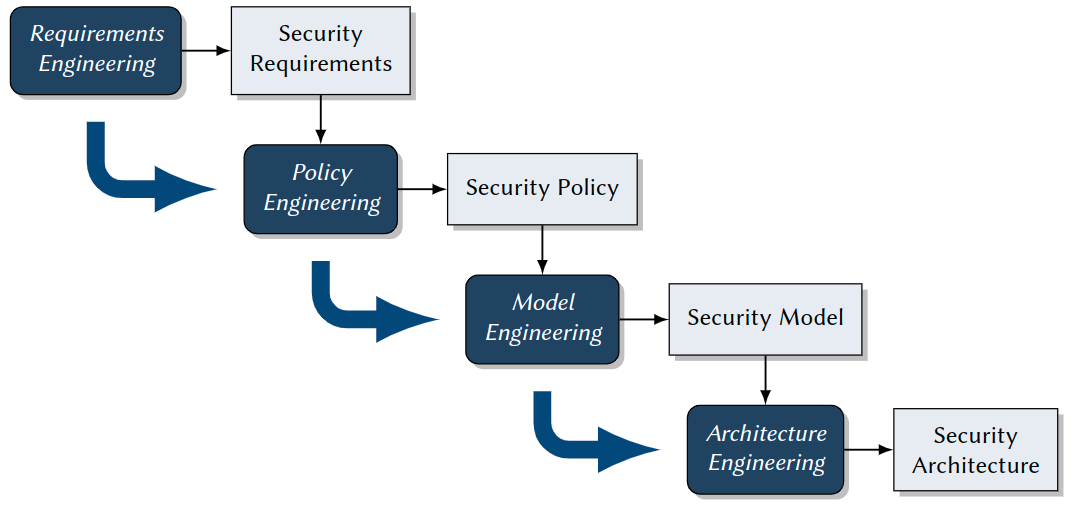
\includegraphics[width=\linewidth]{Assets/Systemsicherheit-engineering-process.png}

    \section{Security Requirements}
    Goal of Requirements Engineering:
    Methodology for identifying and specifying the desired security properties of an IT system.

    Result:
    \begin{itemize*}
        \item Security requirements, which define what security properties a system should have.
        \item These again are the basis of a security policy: Defines how these properties are achieved
    \end{itemize*}

    Influencing Factors
    \begin{itemize*}
        \item Codes and acts (depending on applicable law)
        \begin{itemize*}
            \item EU General Data Protection Regulation (GDPR)
            \item US Sarbanes-Oxley Act (SarbOx)
        \end{itemize*}
        \item Contracts with customers
        \item Certification
        \begin{itemize*}
            \item For information security management systems (ISO 27001)
            \item Subject to German Digital Signature Act (Signaturgesetz)
        \end{itemize*}
        \item Criteria
        \item Company-specific guidelines and regulations
        \begin{itemize*}
            \item Access to critical data
            \item Permission assignment
        \end{itemize*}
        \item Company-specific infrastructure and technical requirements
        \begin{itemize*}
            \item System architecture
            \item Application systems (OSs, Database Information Systems)
        \end{itemize*}
    \end{itemize*}

    General Methodology: How to Come up with Security Requirements

    Specialized steps in regular software requirements engineering:
    \begin{enumerate*}
        \item Identify and classifyvulnerabilities.
        \item Identify and classifythreats.
        \item Match both, where relevant, to yieldrisks.
        \item Analyze and decide which risks should bedealt with.
    \end{enumerate*}
    $\rightarrow$ Fine-grained Security Requirements

    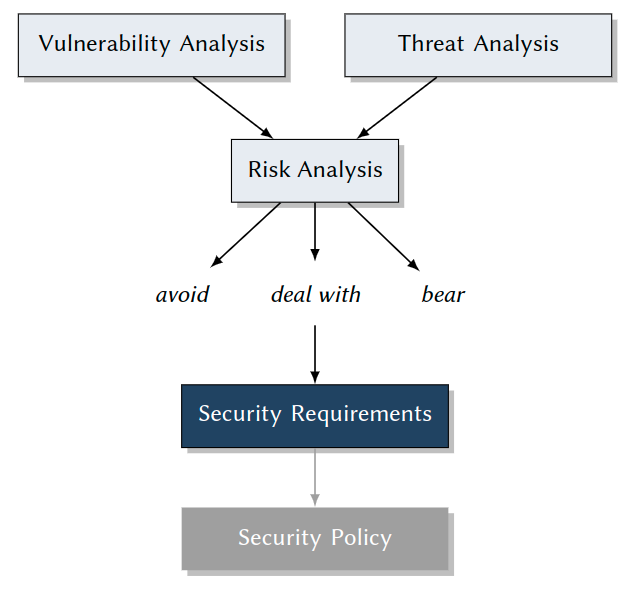
\includegraphics[width=\linewidth]{Assets/Systemsicherheit-risk.png}

    \subsection{Vulnerability Analysis}
    Goal: Identification of
    \begin{itemize*}
        \item technical
        \item organizational
        \item human
    \end{itemize*}
    vulnerabilities of IT systems.

    \note{Vulnerability}{Feature of hardware and software constituting, an organization running, or a human operating an IT system, which is a necessary precondition for any attack in that system, with the goal to compromise one of its security properties. Set of all vulnerabilities = a system’sattack surface.}

    \subsubsection{Human Vulnerabilities}
    \begin{itemize*}
        \item Laziness
        \begin{itemize*}
            \item Passwords on Post-It
            \item Fast-clicking exercise: Windows UAC pop-up boxes
        \end{itemize*}
        \item Social Engineering
        \begin{itemize*}
            \item Pressure from your boss
            \item A favor for your friend
            \item Blackmailing: The poisoned daughter, ...
        \end{itemize*}
        \item Lack of knowledge
        \begin{itemize*}
            \item Importing and executing malware
            \item Indirect, hidden information flowin access control systems
        \end{itemize*}
    \end{itemize*}

    \note{Social Engineering}{Influencing people into acting against their own interest or the interest of an organisation is often a simpler solution than resorting to malware or hacking.
        %Both law enforcement and the financial industry indicate that social engineering continues to enable attackers who lack the technical skills, motivation to use them or the resources to purchase or hire them. Additionally, targeted social engineering allows those technically gifted to orchestrate blended attacks bypassing both human and hardware or software lines of defence.
    }

    \subsubsection{Indirect Information Flow in Access Control Systems}

    \note{Security Requirement}{No internal information about a project, which is not approved by the project manager, should ever go into the product flyer.}

    \note{Forbidden Information Flow}{Internal information about ProjectX goes into the product flyer!}

    Problem Analysis:
    \begin{itemize*}
        \item Limited knowledge of users
        \begin{itemize*}
            \item limited horizon: knowledge about the rest of a system
            \item limited problem awareness: see "lack of knowledge"
            \item limited skills
        \end{itemize*}
        \item Problem complexity $\rightarrow$  effects of individual permission assignments by users to system-wide security properties
        \item Limited configuration options and granularity: archaic and inapt security mechanisms in system and application software
        \begin{itemize*}
            \item no isolation of non-trusted software
            \item no enforcement of global security policies
        \end{itemize*}
        \item $\rightarrow$ Effectiveness of discretionary access control (DAC)
    \end{itemize*}

    \subsubsection{Organizational Vulnerabilities}
    \begin{itemize*}
        \item Access to rooms (servers!)
        \item Assignment of permission on organizational level, e. g.
        \begin{itemize*}
            \item 4-eyes principle
            \item need-to-know principle
            \item definition of roles and hierarchies
        \end{itemize*}
        \item Management of cryptographic keys
    \end{itemize*}

    \subsubsection{Technical Vulnerabilities}
    The Problem: Complexity of IT Systems
    \begin{itemize*}
        \item ... will in foreseeable time not be
        \item Completely, consistently, unambiguously, correctly specified $\rightarrow$  contain specification errors
        \item Correctly implemented $\rightarrow$  contain programming errors
        \item Re-designed on a daily basis $\rightarrow$ contain conceptual weaknesses and vulnerabilities
    \end{itemize*}

    \subsubsection{Buffer Overflow Attacks}
    Privileged software can be tricked into executing attacker’s code.
    Approach: Cleverly forged parameters overwrite procedure activation frames in memory
    \begin{itemize*}
        \item $\rightarrow$ exploitation of missing length checks on input buffers
        \item $\rightarrow$ buffer overflow
    \end{itemize*}
    What an Attacker Needs to Know
    \begin{itemize*}
        \item Source code of the target program, obtained by disassembling
        \item Better: symbol table, as with an executable
        \item Even better: most precise knowledge about the compiler used
        \begin{itemize*}
            \item how call conventions affect the stack layout
            \item degree to which stack layout is deterministic
        \end{itemize*}
    \end{itemize*}
    Sketch of the Attack Approach (Observations during program execution)
    \begin{itemize*}
        \item Stack grows towards the small addresses
        \item in each procedure frame: address of the next instruction to call after the current procedure returns (ReturnIP)
        \item after storing the ReturnIP, compilers reserve stack space for local variables $\rightarrow$ these occupy lower addresses
    \end{itemize*}
    Result
    \begin{itemize*}
        \item Attacker makes victim program overwrite runtime-critical parts of its stack
        \begin{itemize*}
            \item by counting up to the length of msg
            \item at the same time writing back over previously save runtime information $\rightarrow$  ReturnIP
        \end{itemize*}
        \item After finish: victim program executes code at address of ReturnIP (=address of a forged call to execute arbitrary programs)
        \item Additional parameter: file system location of a shell
    \end{itemize*}

    \note{Security Breach}{The attacker can remotely communicate, upload, download, and execute anything- with cooperation of the OS, since all of this runs with the original privileges of the victim program!}

    \subsubsection{Summary - Vulnerabilities}
    \begin{itemize*}
        \item Human
        \begin{itemize*}
            \item Laziness
            \item Social engineering
            \item Lack of knowledge (e.g. malware execution)
        \end{itemize*}
        \item Organizational
        \begin{itemize*}
            \item Key management
            \item Physical access to rooms, hardware
        \end{itemize*}
        \item Technical
        \begin{itemize*}
            \item Weak security paradigms
            \item Specification and implementation errors
        \end{itemize*}
    \end{itemize*}

    \subsection{Threat Analysis}
    Goal: Identification of
    \begin{itemize*}
        \item Attack objectives and attackers
        \item Attack methods and practices (Tactics, Techniques)
        \item $\rightarrow$ know your enemy
    \end{itemize*}

    Approach: Compilation of a threat catalog, content:
    \begin{itemize*}
        \item identified attack objectives
        \item identified potential attackers
        \item identified attack methods \& techniques
        \item damage potential of attacks
    \end{itemize*}

    \subsubsection{Attack Objectives and Attackers}
    \begin{itemize*}
        \item Economic Espionage and political power
        \begin{itemize*}
            \item Victims: high tech industry
            \item Attackers:
            \begin{itemize*}
                \item Competitors, governments, professional organizations
                \item Insiders
                \item regular, often privileged users of IT systems
            \end{itemize*}
            \item often indirect $\rightarrow$ social engineering
            \item statistical profile: age 30-40, executive function
            \item weapons: technical and organisational insider knowledge
            \item damage potential: Loss of control over critical knowledge $\rightarrow$  loss of economical or political power
        \end{itemize*}
        \item Personal Profit
        \begin{itemize*}
            \item Objective: becoming rich(er)
            \item Attackers: Competitors, Insiders
            \item damage potential: Economical damage (loss of profit)
        \end{itemize*}
        \item Wreak Havoc
        \begin{itemize*}
            \item Objective: damaging or destroying things or lives, blackmailing,...
            \item Attackers:
            \begin{itemize*}
                \item Terrorists: motivated by faith and philosophy, paid by organisations and governments
                \item Avengers: see insiders
                \item Psychos: all ages, all types, personality disorder
                \item $\rightarrow$  No regular access to IT systems, no insider knowledge, but skills and tools.
            \end{itemize*}
            \item damage potential: Loss of critical infrastructures
        \end{itemize*}
        \item Meet a challenge (Hackers both good or evil)
    \end{itemize*}

    \subsubsection{Attack Methods}
    Exploitation of Vulnerabilities

    \paragraph{Scenario 1: Insider Attack}
    \begin{itemize*}
        \item Social Engineering
        \item Exploitation of conceptual vulnerabilities (DAC)
        \item Professionally tailored malware
    \end{itemize*}

    \paragraph{Scenario 2: Malware (a family heirloom ...)}
    \begin{itemize*}
        \item Trojan horses: Executable code with hidden functionality
        \item Viruses: Code for self-modification and self-duplication
        \item Logical bombs: Code that is activated by some event recognizable from the host (e. g. time, date, temperature, ...).
        \item Backdoors: Code that is activated through undocumented interfaces (mostly remote).
        \item Ransomware: Code for encrypting possibly all user data found on the host, used for blackmailing the victims
        \item Worms and worm segments: Autonomous, self-duplicating programs
    \end{itemize*}

    \paragraph{Scenario 3: Outsider Attack}
    \begin{itemize*}
        \item Attack Method: Buffer Overflow
        \item Exploitation of implementation errors
    \end{itemize*}

    \paragraph{Scenario 4: High-end Malware (Root Kits)}
    \begin{itemize*}
        \item Invisible, total, sustainable takeover of a complete IT system
        \item Method: Comprehensive tool kit for fully automated attacks
        \begin{enumerate*}
            \item automatic analysis of technical vulnerabilities
            \item automated attack execution
            \item automated installation of backdoors
            \item automated installation and activation of stealth mechanisms
        \end{enumerate*}
        \item Target: Attacks on all levels of the software stack:
        \begin{itemize*}
            \item firmware \& bootloader
            \item operating system (e. g. file system, network interface)
            \item system applications (e. g. file and process managers)
            \item user applications (e. g. web servers, email, office)
        \end{itemize*}
        \item tailored to specific software and software versions found there!
    \end{itemize*}

    \subsubsection{Root Kits}
    Step 1: Vulnerability Analysis
    \begin{itemize*}
        \item Tools look for vulnerabilities in
        \begin{itemize*}
            \item Active privileged services and demons (from inside a network :nmap, from outside: by port scans)
            \item Configuration files $\rightarrow$ Discover weak passwords, open ports
            \item Operating systems $\rightarrow$ Discover kernel and system tool versions with known implementation errors
        \end{itemize*}
        \item built-in knowledge base: automatable vulnerability database
        \item Result: System-specific collection of vulnerabilities $\rightarrow$ choice of attack method and tools to execute
    \end{itemize*}
    Step 2: Attack Execution
    \begin{itemize*}
        \item Fabrication of tailored software to exploit vulnerabilities in
        \begin{itemize*}
            \item Server processes or system tool processes (demons)
            \item OS kernel to execute code of attacker with root privileges
        \end{itemize*}
        \item This code
        \begin{itemize*}
            \item First installs smoke-bombs for obscuring attack
            \item replaces original system software by pre-fabricated modules servers, utilities, libraries, OS modules
            \item containing backdoors or smoke bombs for future attacks
        \end{itemize*}
        \item Results:
        \begin{itemize*}
            \item Backdoors allow for high-privilege access in short time
            \item System modified with attacker’s servers, demons, utilities...
            \item Obfuscation of modifications and future access
        \end{itemize*}
    \end{itemize*}
    Step 3: Attack Sustainability
    \begin{itemize*}
        \item Backdoors for any further control \& command in Servers, ...
        \item Modifications of utilities and OS to prevent
        \begin{itemize*}
            \item Killing root kit processes and connections (kill,signal)
            \item Removal of root kit files (rm,unlink)
        \end{itemize*}
        \item Results: Unnoticed access for attacker anytime, highly privileged, extremely fast, virtually unpreventable
    \end{itemize*}
    Step 4: Stealth Mechanisms (Smoke Bombs)
    \begin{itemize*}
        \item Clean logfiles (entries for root kit processes, network connections), e.g. syslog,kern.log,user.log,daemon.log,auth.log, ...
        \item Modify system admin utilities
        \begin{itemize*}
            \item Process management(hide running root kit processes)
            \item File system (hide root kit files)
            \item Network (hide active root kit connections)
        \end{itemize*}
        \item Substitute OS kernel modules and drivers (hide root kit processes, files, network connections), e.g. /proc/...,stat,fstat,pstat
        \item Result:Processes, files and communication of root kit become invisible
    \end{itemize*}

    Risk and Damage Potential:
    \begin{itemize*}
        \item Likeliness of success: extremely highin today’s commodity OSs (High number of vulnerabilities, Speed, Refined methodology, Fully automated)
        \item Fighting the dark arts: extremely difficult (Number and cause of vulnerabilities, weak security mechanisms, Speed, Smoke bombs)
        \item Prospects for recovering the system after successful attack: near zero
    \end{itemize*}

    Countermeasures - Options:
    \begin{itemize*}
        \item Reactive: even your OS might have become your enemy
        \item Preventive: Counter with same tools for vulnerability analysis
        \item Preventive: Write correct software
    \end{itemize*}

    \note{Security Engineering}{
        \begin{itemize*}
            \item New paradigms: policy-controlled systems $\rightarrow$ powerful software platforms
            \item New provable guarantees: formal security models $\rightarrow$ reducing specification errors and faults by design
            \item New security architectures $\rightarrow$ limiting bad effects of implementation errors and faults
        \end{itemize*}
    }

    \subsection{Risk Analysis}
    Identification and Classification of scenario-specific risks
    \begin{itemize*}
        \item Risks $\subseteq$ Vulnerabilities $\times$ Threats
        \item Correlation of vulnerabilities and threats $\rightarrow$  Risk catalogue
        \item Classification of risks $\rightarrow$ Complexity reduction
        \item $\rightarrow$ Risk matrix
        \item n Vulnerabilities, m Threats $\rightarrow$ x Risks
        \item Correlation of Vulnerabilities and Threats $\rightarrow$ Risk catalogue $n:m$ correlation
        \item $max(n,m)<< x \leq nm$ $\rightarrow$ quite large risk catalogue!
    \end{itemize*}
    Risk Classification: Qualitative risk matrix/dimensions

    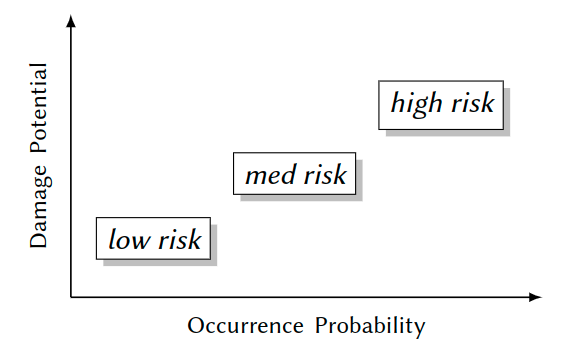
\includegraphics[width=.3\linewidth]{Assets/Systemsicherheit-risk-classification.png}

    \subsubsection{Assessment}
    Damage Potential Assessment
    \begin{itemize*}
        \item Cloud computing $\rightarrow$ loss of confidence/reputation
        \item Industrial plant control $\rightarrow$  damage or destruction of facility
        \item Critical public infrastructure $\rightarrow$  interrupted services, possible impact on public safety
        \item Traffic management $\rightarrow$ maximum credible accident
    \end{itemize*}
    Occurrence Probability Assessment
    \begin{itemize*}
        \item Cloud computing $\rightarrow$  depending on client data sensitivity
        \item Industrial plant control $\rightarrow$  depending on plant sensitivity
        \item Critical public infrastructure $\rightarrow$  depending on terroristic threat level
        \item Traffic management $\rightarrow$  depending on terroristic threat level
    \end{itemize*}

    \note{Damage potential \& Occurrence probability}{is highly scenario-specific}

    Depends on diverse, mostly non-technical side conditions $\rightarrow$  advisory board needed for assessment

    \paragraph{Advisory Board Output Example}
    \begin{tabular}{ l | l | p{.6cm} | p{4cm} }
        Object & Risk (Loss of...) & Dmg. Pot. & Rationale                                                     \\\hline
        PD     & Confidentiality   & med       & Data protection acts                                          \\
        PD     & Confidentiality   & med       & Certified software                                            \\
        PD     & Integrity         & low       & Errors fast and easily detectable and correctable             \\
        PD     & Integrity         & low       & Certified software, small incentive                           \\
        PD     & Availability      & med       & Certified software                                            \\
        PD     & Availability      & low       & Failures up to one week can be tolerated by manual procedures \\
        TCD    & Confidentiality   & high      & Huge financial gain by competitors                            \\
        TCD    & Confidentiality   & high      & Loss of market leadership                                     \\
        TCD    & Integrity         & high      & Production downtime                                           \\
        TCD    & Integrity         & med       & Medium gain by competitors or terroristic attackers           \\
        TCD    & Availability      & low       & Minimal production delay, since backups are available         \\
        TCD    & Availability      & low       & Small gain by competitors or terroristic attackers
    \end{tabular}
    PD = Personal Data; TCD = Technical Control Data

    \begin{multicols*}{2}
        \begin{center}
            Resulting Risk Matrix
            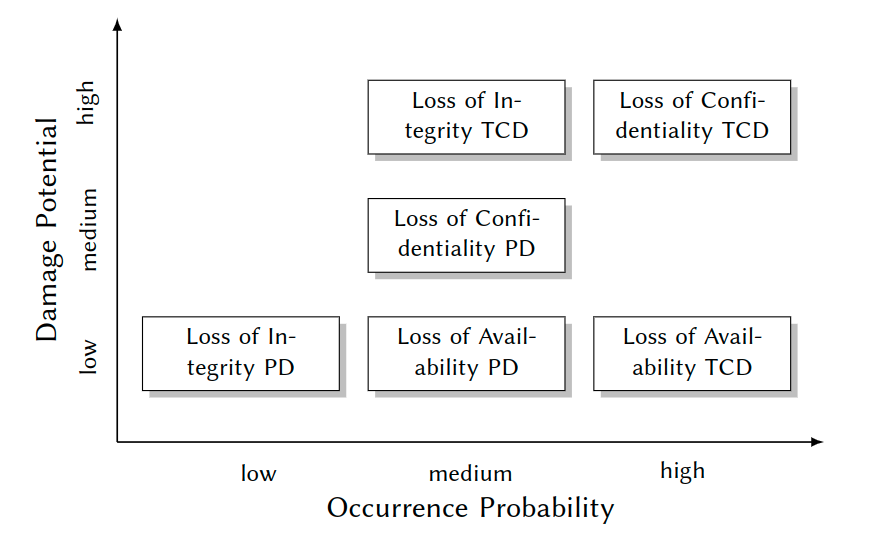
\includegraphics[width=.9\linewidth]{Assets/Systemsicherheit-risk-matrix-1.png}
        \end{center}
        \begin{center}
            Identify 3 Regions
            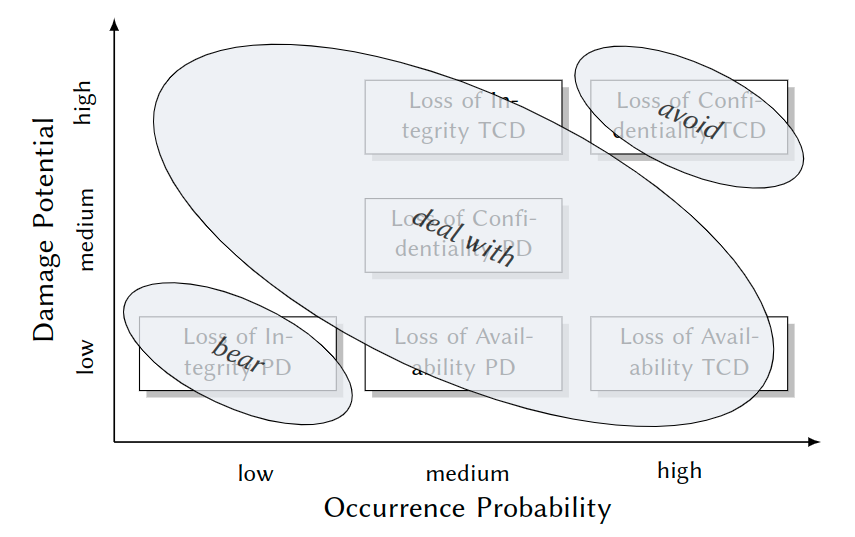
\includegraphics[width=.9\linewidth]{Assets/Systemsicherheit-Risk-Matrix-2.png}
        \end{center}
    \end{multicols*}

    Form Risks to Security Requirements
    \begin{itemize*}
        \item avoid: Intolerable risk, no reasonable proportionality of costs and benefits $\rightarrow$ Don’t implement such functionality!
        \item bear: Acceptable risk $\rightarrow$ Reduce economical damage (insurance)
        \item deal with: Risks that yield security requirements $\rightarrow$ Prevent or control by system-enforced security policies.
    \end{itemize*}

    Additional Criteria:
    \begin{itemize*}
        \item Again, non-technical side conditions may apply:
        \begin{itemize*}
            \item Expenses for human resources and IT
            \item Feasibility from organizational and technological viewpoints
        \end{itemize*}
        \item $\rightarrow$  Cost-benefit ratio:management and business experts involved
    \end{itemize*}

    \section{Security Policies and Models}
    \begin{itemize*}
        \item protect against collisions $\rightarrow$ Security Mechanisms
        \item $\rightarrow$  Competent \& coordinated operation of mechanisms $\rightarrow$  Security Policies
        \item $\rightarrow$  Effectiveness of mechanisms and enforcement of security policies $\rightarrow$  Security Architecture
    \end{itemize*}

    Security Policies: a preliminary Definition
    \begin{itemize*}
        \item We have risks:  Malware attack $\rightarrow$ violation of confidentiality and integrity of patient’s medical records
        \item We infer security requirements: Valid information flows
        \item We design a security policy: Rules for controlling information flows
    \end{itemize*}

    \note{Security Policy}{a set of rules designed to meet a set of security objectives}

    \note{Security Objective}{a statement of intent to counter a given threat or to enforce a given security policy}

    Policy representations:
    \begin{itemize*}
        \item informal (natural language) text
        \item formal model
        \item functional software specification
        \item executable code
    \end{itemize*}

    How to Implement Security Policies
    \begin{itemize*}
        \item (A) Integrated in systems software ( Operating, Database)
        \item (B) Integrated in application systems
    \end{itemize*}

    \subsubsection{Implementation Alternative A}
    The security policy is handled an OS abstractionon its own $\rightarrow$  implemented inside the kernel
    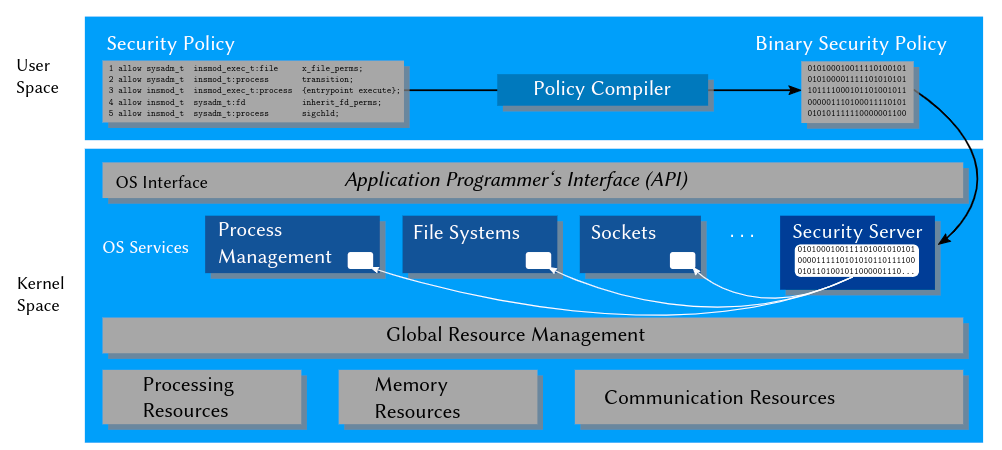
\includegraphics[width=.5\linewidth]{Assets/Systemsicherheit-pos.png}

    Policy Enforcement in SELinux
    \begin{itemize*}
        \item \textbf{Security Server} Policy runtime environment
        \item \textbf{Interceptors} Total control of critical interactions
        \item \textbf{Policy Compiler} Translates human-readable policy modules in kernel-readable binary modules
        \item \textbf{Security Server} Manages and evaluates these modules
    \end{itemize*}

    \subsubsection{Implementation Alternative B}
    \begin{itemize*}
        \item \textbf{Application-embedded Policy} The security policy is only known and enforced by oneuser program $\rightarrow$ implemented in a user-space application
        \item \textbf{Application-level Security Architecture} The security policy is known and enforced by several collaborating user programs in an application systems $\rightarrow$ implemented in a local, user-space security architecture
        \item \textbf{Policy Server Embedded in Middleware} The security policy is communicated and enforced by several collaborating user programs in a distributed application systems $\rightarrow$ implemented in a distributed, user-space security architecture
    \end{itemize*}

    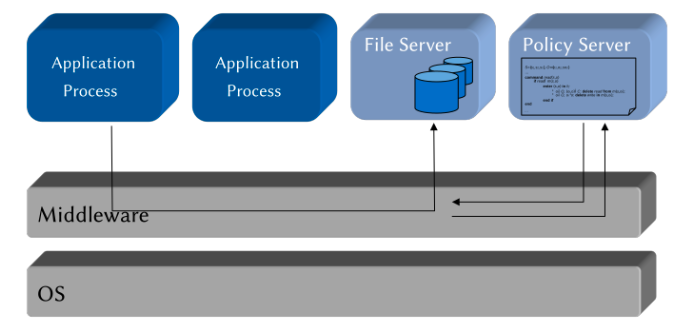
\includegraphics[width=.5\linewidth]{Assets/Systemsicherheit-application-embedded-policy.png}

    \subsection{Security Models}
    Goal of Formal Security Models
    \begin{itemize*}
        \item Complete, unambiguous representation of security policies for
        \item analyzing and explaining its behavior
        \item enabling its correct implementation
    \end{itemize*}

    How We Use Formal Models: Model-based Methodology
    \begin{itemize*}
        \item Abstraction from (usually too complex) reality $\rightarrow$ get rid of insignificant details
        \item Precisionin describing what is significant $\rightarrow$ Model analysis and implementation
    \end{itemize*}

    \note{Security Model}{A security model is a precise, generally formal representation of a security policy.}

    Model Spectrum
    \begin{itemize*}
        \item Models for access control policies:
        \begin{itemize*}
            \item identity-based access control (IBAC)
            \item role-based access control (RBAC)
            \item attribute-based access control (ABAC)
        \end{itemize*}
        \item Models for information flow policies $\rightarrow$ multilevel security (MLS)
        \item Models for non-interference/domain isolation policies $\rightarrow$ non-interference (NI)
        \item In Practice: Most often hybrid models
    \end{itemize*}

    \subsubsection{Access Control Models}
    Formal representations of permissions to execute operations on objects

    Security policies describe access rules $\rightarrow$ security models formalize them Taxonomy
    \note{Identity-based access control models (IBAC)}{Rules based on the identity of individual subjects (users, apps, processes, ...) or objects (files, directories, database tables, ...)}

    \note{Role-based access control models (RBAC)}{Rules based on roles of subjects in an organization}

    \note{Attribute-based access control models (ABAC)}{Rules based on attributes of subjects and objects}

    \note{Discretionary Access Control (DAC)}{Individual users specify access rules to objects within their area of responsibility (at their discretion).}
    Consequence: Individual users
    \begin{itemize*}
        \item granting access permissions as individually needed
        \item need to collectively enforce their organization’s security policy
        \begin{itemize*}
            \item competency problem
            \item responsibility problem
            \item malware problem
        \end{itemize*}
    \end{itemize*}

    \note{Mandatory Access Control (MAC)}{System designers and administrators specify system-wide rules, that apply for all users and cannot be sidestepped.}
    Consequence:
    \begin{itemize*}
        \item Limited individual freedom
        \item Enforced by central instance:
        \begin{itemize*}
            \item clearly identified
            \item competent (security experts)
            \item responsible (organizationally \& legally)
        \end{itemize*}
    \end{itemize*}

    \paragraph{DAC vs. MAC}
    In Real-world Scenarios: Mostly hybrid models enforced by both discretionary and mandatory components
    \begin{itemize*}
        \item \textbf{DAC} locally within a project, team members individually define permissions w. r. t. documents inside this closed scope
        \item \textbf{MAC} globally for the organization, such that e. g. only documents approved for release by organizational policy rules may be accessed from outside a project’s scope
    \end{itemize*}

    \paragraph{Identity-based Access Control Models (IBAC)}
    To precisely specify the rights of individual, acting entities.
    \begin{center}
        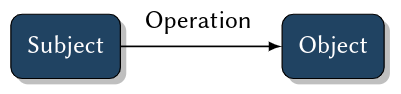
\includegraphics[width=.5\linewidth]{Assets/Systemsicherheit-ibac-basic.png}
    \end{center}
    There are
    \begin{itemize*}
        \item \textbf{Subjects}, i.e. active and identifiable entities, that execute
        \item \textbf{Operations} on
        \item passive and identifiable \textbf{Objects}, requiring
        \item \textbf{Rights} (also: permissions, privileges) which
        \begin{itemize*}
            \item control (restrict) execution of operations,
            \item are checked against identity of subjects and objects.
        \end{itemize*}
    \end{itemize*}

    Access Control Functions [Lampson, 1974]
    \begin{itemize*}
        \item A really basic model to define access rights:
        \begin{itemize*}
            \item Who (subject) is allowed to do what (operation) on which object
            \item Fundamental to OS access control since 1965
            \item Formal paradigms: sets and functions
        \end{itemize*}
        \item Access Control Function (ACF)
        \begin{itemize*}
            \item $f:S \times O \times OP \rightarrow \{true,false\}$ where
            \item S is a set of subjects (e. g. users, processes),
            \item O is a set of objects(e. g. files, sockets),
            \item OP is a finite set of operations(e. g. read, write, delete)
        \end{itemize*}
        \item Interpretation: Rights to execute operations are modeled by ACF
        \begin{itemize*}
            \item any $s\in S$ represents an authenticated active entity which potentially executes operations on objects
            \item any $o\in O$ represents an authenticated passive entity on which operations are executed
            \item for any $s\in S$,$o\in O$,$op\in OP$:s is allowed to execute $op$ on $o$ iff $f(s,o,op)=true$.
            \item Model making: finding a $tuple\langle S,O,OP,f\rangle$
        \end{itemize*}
    \end{itemize*}

    \paragraph{Access Control Matrix}
    Lampson [1974] addresses the questions how to ...
    \begin{itemize*}
        \item store in a well-structured way,
        \item efficiently evaluate and
        \item completely analyze an ACF
    \end{itemize*}

    \note{Access Control Matrix (ACM)}{An ACM is a matrix $m:S\times O \rightarrow 2^{OP}$, such that $\forall s\in S,\forall o\in O:op\in m(s,o)\Leftrightarrow f(s,o,op)$.}

    An ACM is a rewriting of the definition of an ACF: nothing is added, nothing is left out ("$\Leftrightarrow$"). Despite a purely theoretical model: paved the way for practically implementing AC meta-information as tables, 2-dimensional lists, distributed arrays and lists.

    Example
    \begin{itemize*}
        \item $S=\{s_1 ,...,s_n\}$
        \item $O=\{o_1 ,...,o_k\}$
        \item $OP=\{read,write\}$
        \item $2^{OP}=\{\varnothing,\{read\},\{write\},\{read,write\}\}^2$
        %![](Assets/Systemsicherheit-access-control-matrix.png)
    \end{itemize*}

    Implementation Notes
    \begin{itemize*}
        \item ACMs are implemented in most OS, DB, Middlewear
        \item whose security mechanisms use one of two implementations
    \end{itemize*}

    Access Control Lists (ACLs)
    \begin{itemize*}
        \item Columns of the ACM: $char*o3[N]=\{ '-', '-', 'rw', ...\};$
        \item Found in I-Nodes of Unix(oids), Windows, Mac OS
    \end{itemize*}

    Capability Lists
    \begin{itemize*}
        \item Rows of the ACM: $char* s1[K]=\{'-', 'r', '-', ...\};$
        \item Found in distributed OSs, middleware, Kerberos
    \end{itemize*}

    What we actually Model:
    \note{Protection State}{A fixed-time snapshot of all active entities, passive entities, and any meta-information used for making access decisions is called theprotection state of an access control system.}

    Goal of ACF/ACM is to precisely specify a protection state of an AC system.

    \paragraph{The Harrison-Ruzzo-Ullman Model (HRU)}

    Privilege escalation question: "Can it ever happen that in a given state, some specific subject obtains a specific permission?"
    $\varnothing \Rightarrow \{r,w\}$
    \begin{itemize*}
        \item ACM models a single state $\langle S,O,OP,m\rangle$
        \item ACM does not tell anything about what might happen in future
        \item Behavior prediction $\rightarrow$  proliferation of rights $\rightarrow$ HRU safety
    \end{itemize*}

    We need a model which allows statements about
    \begin{itemize*}
        \item Dynamic behavior of right assignments
        \item Complexity of such an analysis
    \end{itemize*}

    Idea [Harrison et al., 1976]: A (more complex) security model combining
    \begin{itemize*}
        \item Lampson’s ACM $\rightarrow$  for modeling single protection state (snapshots) of an AC system
        \item Deterministic automata (state machines) $\rightarrow$  for modeling runtime changes of a protection state
    \end{itemize*}

    This idea was pretty awesome. We need to understand automata, since from then on they were used for most security models.

    \paragraph{Deterministic Automata}
    Mealy Automat $(Q,\sum,\Omega,\delta,\lambda,q_0)$
    \begin{itemize*}
        \item $Q$ is a finite set of states, e. g. $Q=\{q_0 ,q_1 ,q_2\}$
        \item $\sum$ is a finite set of input words, e. g. $\sum=\{a,b\}$
        \item $\Omega$ is a finite set of output words, e. g. $\Omega=\{yes,no\}$
        \item $\delta:Q\times\sum\rightarrow Q$ is the state transition function
        \item $\lambda:Q\times\sum\rightarrow\Omega$ is the output function
        \item $q_0\in Q$ is the initial state
        \item $\delta(q,\sigma)=q'$ and $\lambda(q,\sigma)=\omega$ can be expressed through the state diagram
    \end{itemize*}

    \paragraph{HRU Security Model}
    How we use Deterministic Automata
    \begin{itemize*}
        \item Snapshot of an ACM is the automaton’s state
        \item Changes of the ACM during system usage are modeled by state transitions of the automaton
        \item Effects of operations that cause such transitions are described by the state transition function
        \item Analyses of right proliferation ($\rightarrow$  privilege escalation) are enabled by state reachability analysis methods
    \end{itemize*}

    An HRU model is a deterministic automaton $\langle Q,\sum,\delta,q_0 ,R\rangle$ where
    \begin{itemize*}
        \item $Q= 2^S\times 2^O\times  M$ is the state space where
        \begin{itemize*}
            \item S is a (not necessarily finite) set of subjects,
            \item O is a (not necessarily finite) set of objects,
            \item $M=\{m|m:S\times O\rightarrow 2^R\}$ is a set of possible ACMs,
        \end{itemize*}
        \item $\sum=OP\times X$ is the (finite) input alphabet where
        \begin{itemize*}
            \item $OP$ is a set of operations,
            \item $X=(S\cup O)^k$ is a set of k-dimensional vectors of arguments (subjects or objects) of these operations,
        \end{itemize*}
        \item $\sigma:Q\times\sum\rightarrow Q$ is the state transition function,
        \item $q_0\in Q$ is the initial state,
        \item R is a (finite) set of access rights.
    \end{itemize*}

    Interpretation
    \begin{itemize*}
        \item Each $q=S_q,O_q,m_q\in Q$ models a system’s protection state:
        \begin{itemize*}
            \item current subjects set $S_q\subseteq S$
            \item current objects set $O_q\subseteq O$
            \item current ACM $m_q\in M$ where $m_q:S_q\times O_q\rightarrow 2^R$
        \end{itemize*}
        \item State transitions modeled by $\delta$ based on
        \begin{itemize*}
            \item the current automaton state
            \item an input word $\langle op,(x_1,...,x_k)\rangle \in\sum$ where $op$
            \item may modify $S_q$ (create a user $x_i$),
            \item may modify $O_q$ (create/delete a file $x_i$),
            \item may modify the contents of a matrix cell $m_q(x_i,x_j)$ (enter or remove rights) where $1\leq i,j\leq k$.
            \item $\rightarrow$  We also call $\delta$ the state transition scheme (STS) of a model.
            \item Historically: "authorization scheme" [Harrison et al., 1976].
        \end{itemize*}
    \end{itemize*}

    \paragraph{State Transition Scheme (STS)}
    Using the STS, $\sigma:Q\times\sum\rightarrow Q$ is defined by a set of specifications in the normalized form
    $\sigma(q,\langle op,(x_1,...,x_k)\rangle )$=if $r_1\in m_q(x_{s1},x_{o1}) \wedge ... \wedge r_m\in m_q(x_{sm},x_{om})$ then $p_1\circ ...\circ p_n$ where
    \begin{itemize*}
        \item $q=\{S_q,O_q,m_q\}\in Q,op\in OP$
        \item $r_1 ...r_m\in R$
        \item $x_{s1},...,x_{sm}\in S_q$ and $x_{o1},...,x_{om}\in O_q$ where $s_i$ and $o_i$, $1\leq i\leq m$, are vector indices of the input arguments: $1\leq s_i,o_i\leq k$
        \item $p_1,...,p_n$ are HRU primitives
        \item $\circ$ is the function composition operator: $(f\circ g)(x)=g(f(x))$
    \end{itemize*}

    Conditions: Expressions that need to evaluate "true" for state q as a necessary precondition for command $op$ to be executable (= can be successfully called).

    Primitives: Short, formal macros that describe differences between $q$ and $a$ successor state $q'=\sigma(q,\langle op,(x_1 ,...,x_k)\rangle )$ that result from a complete execution of op:
    \begin{itemize*}
        \item enter r into $m(x_s,x_o)$
        \item delete r from $m(x_s,x_o)$
        \item create subject $x_s$
        \item create object $x_o$
        \item destroy subject $x_s$
        \item destroy object $x_o$
        \item Each above with semantics for manipulating $S_q, O_q$ or $m_q$.
    \end{itemize*}

    Note the atomic semantics: the HRU model assumes that each command successfully called is always completely executed!

    How to Design an HRU Security Model:
    \begin{enumerate*}
        \item  Model Sets: Subjects, objects, operations, rights $\rightarrow$  define the basic sets $S,O,OP,R$
        \item STS: Semantics of operations (e. g. the future API of the system to model) that modify the protection state $\rightarrow$  define $\sigma$ using the normalized form/programming syntax of the STS
        \item Initialization: Define a well-known initial stateq $0 =\langle S_0 ,O_0 ,m_0 \rangle$ of the system to model
    \end{enumerate*}

    1. Model Sets
    \begin{itemize*}
        \item Subjects, objects, operations, rights:
        \begin{itemize*}
            \item Subjects: An unlimited number of possible students: $S\cong\mathbb{N}$
            \item Objects: An unlimited number of possible solutions: $O\cong\mathbb{N}$
            \item Operations:
            \begin{itemize*}
                \item (a) Submit $writeSolution(s_{student},o_{solution})$
                \item (b) Download $readSample(s_{student},o_{sample})$
                \item $\rightarrow OP=\{writeSolution, readSample\}$
            \end{itemize*}
            \item Rights: Exactly one allows to execute each operation
            \begin{itemize*}
                \item $R\cong OP$ $\rightarrow R=\{write, read\}$
            \end{itemize*}
        \end{itemize*}
    \end{itemize*}
    2. State Transition Scheme: Effects of operations on protection state
    \begin{lstlisting}[language=Bash,showspaces=false]
        command writeSolution(s,o) ::= if write in m(s,o) 
          then 
            enter read into m(s,o);
          fi
        command readSample(s,o) ::= if read in m(s,o)
          then
            delete write from m(s,o);
          fi
  \end{lstlisting}
    3. Initialization
    \begin{itemize*}
        \item By model definition: $q_0 =\langle S_0 ,O_0 ,m_0 \rangle$
        \item For a course with (initially) three students:
        \begin{itemize*}
            \item $S_0 =\{sAnn, sBob, sChris\}$
            \item $O_0 =\{oAnn, oBob, oChris\}$
            \item $m_0$:
            \begin{itemize*}
                \item $m_0(sAnn,oAnn)=\{write\}$
                \item $m_0(sBob,oBob)=\{write\}$
                \item $m_0(sChris,oChris)=\{write\}$
                \item $m_0(s,o)=\varnothing \Leftrightarrow s\not= o$
            \end{itemize*}
            \item Interpretation: "There is a course with three students, each of whom has their own workspace to which she is allowed to submit (write) a solution."
        \end{itemize*}
    \end{itemize*}

    Model Behavior
    \begin{itemize*}
        \item Initial Protection State at beginning
        \begin{center}\begin{tabular}{l|l|l|l}
                m      & oAnn          & oBob          & oChris        \\\hline
                sAnn   & {write}       & $\varnothing$ & $\varnothing$ \\
                sBob   & $\varnothing$ & {write}       & $\varnothing$ \\
                sChris & $\varnothing$ & $\varnothing$ & {write}
            \end{tabular}\end{center}
        \item After $writeSolution(sChris, oChris)$
        \begin{center}\begin{tabular}{l|l|l|l}
                m      & oAnn          & oBob          & oChris        \\\hline
                sAnn   & {write}       & $\varnothing$ & $\varnothing$ \\
                sBob   & $\varnothing$ & {write}       & $\varnothing$ \\
                sChris & $\varnothing$ & $\varnothing$ & {write, read}
            \end{tabular}\end{center}
        \item After $readSample(sChris, oChris)$
        \begin{center}\begin{tabular}{l|l|l|l}
                m      & oAnn          & oBob          & oChris        \\\hline
                sAnn   & {write}       & $\varnothing$ & $\varnothing$ \\
                sBob   & $\varnothing$ & {write}       & $\varnothing$ \\
                sChris & $\varnothing$ & $\varnothing$ & {read}
            \end{tabular}\end{center}
    \end{itemize*}

    Summary: Model Behavior
    \begin{itemize*}
        \item The model’s input is a sequence of actions from OP together with their respective arguments.
        \item The automaton changes its state according to the STS and the semantics of HRU primitives.
        \item In the initial state, each student may (repeatedly) submit her respective solution.
    \end{itemize*}
    Tricks in this Example
    \begin{itemize*}
        \item The sample solution is not represented by a separate object $\rightarrow$ no separate column in the ACM.
        \item Instead, we smuggled the read right for it into the cell of each student’s solution ...
    \end{itemize*}

    \paragraph{HRU Model Analysis}
    Analysis of Right Proliferation $\rightarrow$  The HRU safety problem.

    InputSequences
    \begin{itemize*}
        \item ,,What is the effect of an input in a given state?'' $\rightarrow$  a single state transition as defined by $\delta$
        \item ,,What is the effect of an input sequence in a given state?'' $\rightarrow$  a composition of sequential state transitions as defined by $\delta*$
    \end{itemize*}

    \note{Transitive State Transition Function $\delta^*$:}{Let $\sigma\sigma\in\sum^*$ be a sequence of inputs consisting of a single input $\sigma\in\sum\cup\{\epsilon\}$ followed by a sequence $\sigma\in\sum^*$, where $\epsilon$ denotes an empty input sequence. Then, $\delta^*:Q\times\sum^*\rightarrow Q$ is defined by
        \begin{itemize*}
            \item $\delta^*(q,\sigma\sigma^*)=\delta^*(\delta(q,\sigma),\sigma^*)$
            \item $\delta^*(q,\epsilon)=q$.
        \end{itemize*}
    }

    \note{HRU Safety}{(also simple-safety) A state q of an HRU model is called HRU safe with respect to a right $r\in R$ iff, beginning with q, there is no sequence of commands that enters r in an ACM cell where it did not exist in q.}

    According to Tripunitara and Li, simple-safety is defined as:

    \note{HRU Safety}{For a state $q=\{S_q,O_q,m_q\}\in Q$ and a right $r\in R$ of an HRU model $\langle Q,\sum,\delta,q_0,R\rangle$, the predicate $safe(q,r)$ holds iff
    $\forall q'= S_{q'},O_{q'},m_{q'} \in \{\delta^*(q,\sigma^*)|\sigma^*\in\sum^*\},\forall s\in S_{q'},\forall o\in O_{q'}: r\in m_{q'}(s,o)\Rightarrow s\in S_q \wedge o\in O_q \wedge r\in m_q(s,o)$.
    We say that an HRU model is safe w.r.t. r iff $safe(q_0 ,r)$.}

    all states in $\{\delta^*(q,\sigma^*)|\sigma^*\in\sum^*\}$ validated except for $q'$
    \begin{tabular}{l|l|l|l}
        $m_q$ & $o_1$         & $o_2$         & $o_3$     \\\hline
        $s_1$ & $\{r_1,r_3\}$ & $\{r_1,r_3\}$ & $\{r_2\}$ \\
        $s_2$ & $\{r_1\}$     & $\{r_1\}$     & $\{r_2\}$ \\
        $s_3$ & $\varnothing$ & $\varnothing$ & $\{r_2\}$
    \end{tabular}
    \begin{tabular}{l|l|l|l|l}
        $m_{q'}$ & $o_1$         & $o_2$         & $o_3$         & $o_4$         \\\hline
        $s_1$    & $\{r_1,r_3\}$ & $\{r_1\}$     & $\{r_2\}$     & $\varnothing$ \\
        $s_2$    & $\{r_1,r_2\}$ & $\{r_1\}$     & $\{r_2\}$     & $\{r_2\}$     \\
        $s_3$    & $\varnothing$ & $\varnothing$ & $\varnothing$ & $\varnothing$
    \end{tabular}
    \begin{itemize*}
        \item $r_3\not\in m_{q'}(s_1,o_2)\wedge r_3\in m_q(s_1,o_1)\Rightarrow safe(q,r_3)$
        \item $r_2\in m_{q'}(s_2,o_1)\wedge r_2 \not\in m_q(s_2,o_1)\Rightarrow\lnot safe(q,r_2)$
        \item $r_2\in m_{q'}(s_2,o_4)\wedge o_4\not\in O_q\Rightarrow\lnot safe(q,r_2)$
    \end{itemize*}

    showing that an HRU model is safe w.r.t. r means to
    \begin{enumerate*}
        \item Search for any possible (reachable) successor state $q'$ of $q_0$
        \item Visit all cells in $m_{q'}$ ($\forall s\in S_{q'},\forall o\in O_{q'}:...$)
        \item If r is found in one of these cells ($r\in m_{q'}(s,o)$), check if
        \begin{itemize*}
            \item $m_q$ is defined for this very cell ($s\in S_q\wedge o\in O_q$),
            \item $r$ was already contained in this very cell in $m_q$ ($r\in m_q...$).
        \end{itemize*}
        \item Recursiv. proceed with 2. for any possible successor state $q''$ of $q'$
    \end{enumerate*}

    Safety Decidability
    \note{Theorem 1 [Harrison]}{Ingeneral, HRU safety is not decidable.}

    \note{Theorem 2 [Harrison]}{For mono-operational models, HRU safety is decidable.}
    \begin{itemize*}
        \item Insights into the operational principles modeled by HRU models
        \item Demonstrates a method to prove safety property for a particular, given model
        \item $\rightarrow$ ,,Proofs teach us how to build things so nothing more needs to be proven.'' (W. E. Kühnhauser)
    \end{itemize*}

    a mono-operational HRU model $\rightarrow$  exactly one primitive for each operation in the STS

    \paragraph{Proof of Theorem - Proof Sketch}
    \begin{enumerate*}
        \item Find an upper bound for the length of all input sequences with different effects on the protection state w.r.t. safety
        If such can be found: $\exists$ a finite number of input sequences with different effects
        \item All these inputs can be tested whether they violate safety. This test terminates because:
        \begin{itemize*}
            \item each input sequence is finite
            \item there is only a finite number of relevant sequences
        \end{itemize*}
        \item $\rightarrow$ safety is decidable
    \end{enumerate*}

    Proof:
    \begin{itemize*}
        \item construct finite sequences ...$\rightarrow$
        \item Transform $\sigma_1...\sigma_n$ into shorter sequences
        \begin{enumerate*}
            \item Remove all input operations that contain delete or destroy primitives (no absence, only presence of rights is checked).
            \item Prepend the sequence with an initial create subject $s_{init}$ operation.
            \item Prune the last create subject s operation and substitute each following reference to s with $s_{init}$. Repeat until all create subject operations are removed, except from the initial create subject $s_{init}$.
            \item Same as steps 2 and 3 for objects.
            \item Remove all redundant enter operations.
        \end{enumerate*}
    \end{itemize*}

    \begin{tabular}{l|l}
        init                       & 5.                                    \\\hline
        ...                        & create subject $s_{init}$;            \\
        ...                        & create object $o_{init}$              \\
        create subject $x2;$       & -                                     \\
        create object $x5;$        & -                                     \\
        enter r1 into $m(x2,x5);$  & enter r1 into $m(s_{init},o_{init})$; \\
        enter r2 into $m(x2,x5);$  & enter r2 into $m(s_{init},o_{init})$; \\
        create subject $x7;$       & -                                     \\
        delete r1 from $m(x2,x5)$; & -                                     \\
        destroy subject $x2;$      & -                                     \\
        enter r1 into $m(x7,x5);$  & -
    \end{tabular}

    Conclusions from these Theorems (Dilemma)
    \begin{itemize*}
        \item General (unrestricted) HRU models
        \begin{itemize*}
            \item have strong expressiveness $\rightarrow$  can model a broad range of AC policies
            \item are hard to analyze: algorithms and tools for safety analysis
        \end{itemize*}
        \item Mono-operational HRU models
        \begin{itemize*}
            \item have weak expressiveness $\rightarrow$ goes as far as uselessness (only create files)
            \item are efficient to analyze: algorithms and tools for safety analysis
            \item $\rightarrow$ are always guaranteed to terminate
            \item $\rightarrow$ are straight-forward to design
        \end{itemize*}
    \end{itemize*}

    \paragraph{(A) Restricted Model Variants}

    Static HRU Models
    \begin{itemize*}
        \item Static: no create primitives allowed
        \item safe(q,r) decidable, but NP-complete problem
        \item Applications: (static) real-time systems, closed embedded systems
    \end{itemize*}

    Monotonous Mono-conditional HRU Models
    \begin{itemize*}
        \item Monotonous (MHRU): no delete or destroy primitives
        \item Mono-conditional: at most one clause in conditions part
        \item safe(q,r) efficiently decidable
        \item Applications: Archiving/logging systems (nothing is ever deleted)
    \end{itemize*}

    Finite Subject Set
    \begin{itemize*}
        \item $\forall q\in Q,\exists n\in N: |S_q|\leq n$
        \item $safe(q,r)$ decidable, but high computational complexity
    \end{itemize*}

    Fixed STS
    \begin{itemize*}
        \item All STS commands are fixed, match particular application domain (e.g. OS access control) $\rightarrow$  no model reusability
        \item For Lipton and Snyder [1977]: $safe(q,r)$ decidable in linear time
    \end{itemize*}

    Strong Type System
    \begin{itemize*}
        \item Special model to generalize HRU: Typed Access Matrix (TAM)
        \item $safe(q,r)$ decidable in polynomial time for ternary, acyclic, monotonous variants
        \item high, though not unrestricted expressiveness in practice
    \end{itemize*}

    \paragraph{(B) Heuristic Analysis Methods}
    \begin{itemize*}
        \item Restricted model variants often too weak for real-world apps
        \item General HRU models: safety property cannot be guaranteed
        \item $\rightarrow$ get a piece from both: Heuristically guided safety estimation
    \end{itemize*}

    Idea:
    \begin{itemize*}
        \item State-space exploration by model simulation
        \item Task of heuristic: generating input sequences (,,educated guessing'')
    \end{itemize*}

    Outline: Two-phase-algorithm to analyze $safe(q_0,r)$:
    \begin{enumerate*}

        \item Static phase: knowledge from model to make "good" decisions
        \begin{itemize*}
            \item $\rightarrow$  Runtime: polynomial in model size ($q_0 + STS$)
        \end{itemize*}
        \item Simulation phase: The automaton is implemented and, starting with $q_0$, fed with inputs $\sigma=<op,x>$
        \begin{itemize*}
            \item $\rightarrow$  For each $\sigma$, the heuristic has to decide:
            \item which operation $op$ to use
            \item which vector of arguments $x$ to pass
            \item which $q_i$ to use from the states in $Q$ known so far
            \item Termination: As soon as $\sigma(q_i,\sigma)$ violates $safe(q_0,r)$.
        \end{itemize*}
    \end{enumerate*}

    Goal: Iteratively build up the $Q$ for a model to falsify safety by example (finding a violating but possible protection state).

    \begin{itemize*}
        \item Termination: only a semi-decidable problem here. It can be guaranteed that a model is unsafe if we terminate. We cannot ever prove the opposite $\rightarrow$ safety undecidability
        \item Performance: Model size 10 000 000 $\approx 417$s
    \end{itemize*}

    Achievements
    \begin{itemize*}
        \item Find typical errors in security policies: Guide designers, who might know there’s something wrong w. r. t. right proliferation, but not what and why!
        \item Increase our understanding of unsafety origins: By building clever heuristics, we started to understand how we might design specialized HRU models ($\rightarrow$ fixed STS, type system) that are safety-decidable yet practically (re-) usable
    \end{itemize*}

    \paragraph{Summary HRU Models}
    Goal
    \begin{itemize*}
        \item Analysis of right proliferation in AC models
        \item Assessing the computational complexity of such analyses
    \end{itemize*}

    Method
    \begin{itemize*}
        \item Combining ACMs and deterministic automata
        \item Defining $safe(q,r)$ based on this formalism
    \end{itemize*}

    Conclusions
    \begin{itemize*}
        \item Potential right proliferation: Generally undecidable problem
        \item $\rightarrow$ HRU model family, consisting of application-tailored, safety-decidable variants
        \item $\rightarrow$ Heuristic analysis methods for practical error-finding
    \end{itemize*}

    \paragraph{The Typed-Access-Matrix Model (TAM)}
    \begin{itemize*}
        \item AC model, similar expressiveness to HRU
        \item $\rightarrow$ directly mapped to implementations of an ACM (DB table)
        \item Better suited for safety analyses: precisely statemodel properties for decidable safety
    \end{itemize*}

    Idea
    \begin{itemize*}
        \item Adopted from HRU: subjects, objects, ACM, automaton
        \item New: leverage the principle of strong typing (like programming)
        \item $\rightarrow$  safety decidability properties relate to type-based restrictions
    \end{itemize*}

    How it Works:
    \begin{itemize*}
        \item Foundation of a TAM model is an HRU model $\langle Q,\sum,\delta,q_0 ,R\rangle$, where $Q= 2^S\times 2^O\times M$
        \item However: $S\subseteq O$, i. e.:
        \begin{itemize*}
            \item all subjects can also act as objects (=targets of an access)
            \item useful for modeling e.g. delegation
            \item objects in $O\backslash S$: pure objects
        \end{itemize*}
        \item Each $o\in O$ has a type from a type set $T$ assigned through a mapping $type:O\rightarrow T$
        \item An HRU model is a special case of a TAM model:
        \begin{itemize*}
            \item $T=\{tSubject,tObject\}$
            \item $\forall s\in S:type(s)=tSubject; \forall o\in O\backslash S:type(o)=tObject$
        \end{itemize*}
    \end{itemize*}

    \note{TAM Security Model}{A TAM model is a deterministic automaton $\langle Q,\sum,\delta,q_0 ,T,R\rangle$ where
        \begin{itemize*}
            \item $Q= 2^S\times 2^O\times TYPE\times M$ is the state space where $S$ and $O$ are subjects set and objects set as in HRU, where $S\subseteq O$, $TYPE=\{type|type:O\rightarrow T\}$ is a set of possible type functions, $M$ is the set of possible $ACMs$ as in HRU,
            \item $\sum=OP\times X$ is the (finite) input alphabet where $OP$ is a set of operations as in HRU, $X=O^k$ is a set of $k$-dimensional vectors of arguments (objects) of these operations,
            \item $\delta:Q\times\sum\rightarrow Q$ is the state transition function,
            \item $q_0\in Q$ is the initial state,
            \item $T$ is a static (finite) set of types,
            \item $R$ is a (finite) set of access rights.
        \end{itemize*}
    }

    State Transition Scheme (STS)
    $\delta:Q\times\sum\rightarrow Q$ is defined by a set of specifications:
    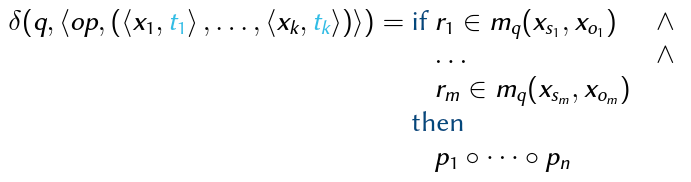
\includegraphics[width=\linewidth]{Assets/Systemsicherheit-tam-sts.png}
    where
    \begin{itemize*}
        \item $q= (S_q,O_q,type_q,m_q)\in Q,op\in OP$
        \item $r_1,...,r_m\in R$
        \item $x_{s1},...,x_{sm}\in S_q,x_{o1},...,x_{om}\in Oq\backslash S_q$, and $t_1,...,t_k\in T$ where $s_i$ and $o_i, 1\leq i\leq m$ , are vector indices of the input arguments: $1\leq s_i,o_i\leq k$
        \item $p_1,...,p_n$ are TAM primitives
    \end{itemize*}

    Convenience Notation where
    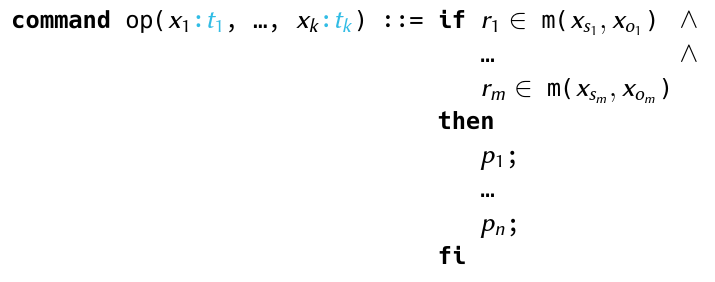
\includegraphics[width=.5\linewidth]{Assets/Systemsicherheit-tam-sts-convenience.png}
    \begin{itemize*}
        \item $q\in Q$ is implicit
        \item $op,r_1 ,...,r_m,s_1 ,...,s_m,o_1 ,...,o_m$ as before
        \item $t_1 ,...,t_k$ are argument types
        \item $p_1 ,...,p_n$ are TAM-specific primitives
    \end{itemize*}

    TAM-specific
    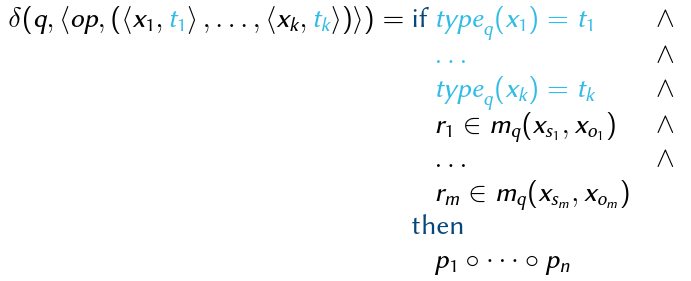
\includegraphics[width=.5\linewidth]{Assets/Systemsicherheit-tam-sts-specific.png}
    \begin{itemize*}
        \item Implicit Add-on:Type Checking
        \item where $t_i$ are the types of the arguments $x_i, 1\leq i\leq k$.
    \end{itemize*}

    TAM-specific
    \begin{itemize*}
        \item Primitives:
        \begin{itemize*}
            \item enter r into m($x_s$,$x_o$)
            \item delete r from m($x_s$,$x_o$)
            \item create subject $x_s$ of type $t_s$
            \item create object $x_o$ of type $t_o$
            \item destroy subject $x_s$
            \item destroy object $x_o$
        \end{itemize*}
        \item Observation: $S$ and $O$ are dynamic (as in HRU), thus $type:O\rightarrow T$ must be dynamic too (cf. definition of $Q$ in TAM).
    \end{itemize*}

    TAM Example: The ORCON Policy
    \begin{itemize*}
        \item Creator/owner of a document should permanently retain controlover its accesses
        \item Neither direct nor indirect (by copying) right proliferation
        \item Application scenarios: Digital rights management, confidential sharing
        \item Solution with TAM: A confined subject type that can never execute any operation other than reading
    \end{itemize*}

    Model Behavior (STS): The State Transition Scheme
    \begin{itemize*}
        \item $createOrconObject(s_1:s, o_1:co)$
        \item $grantCRead(s 1 :s,s 2 :s,o 1 :co)$
        \item $useCRead(s_1:s, o_1:co, s_2:cs)$
        \item $revokeCRead(s_1:s, s_2:s, o_1:co)$
        \item $destroyOrconObject(s_1:s, o_1:co)$ (destroy conf. object)
        \item $revokeRead(s_1:s, s_2:cs, o_1:co)$ (destroy conf. subject)
        \item $finishOrconRead(s_1:s, s_2:cs)$ (destroy conf. subject)
    \end{itemize*}

    \begin{itemize*}
        \item Owner retains full control over
        \item Use of her confined objects by third parties $\rightarrow$ transitive right revocation
        \item Subjects using these objects $\rightarrow$ destruction of these subjects
        \item Subjects using such objects are confined: cannot forward read information
    \end{itemize*}

    \paragraph{TAM Safety Decidability}
    \begin{itemize*}
        \item General TAM models $\rightarrow$ safety not decidable
        \item MTAM: monotonous TAM models; STS without delete or destroy primitives $\rightarrow$ safety decidable if mono-conditional only
        \item AMTAM: acyclic MTAM models $\rightarrow$ safety decidable but not efficiently (NP-hard problem)
        \item TAMTAM: ternary AMTAM models; each STS command requires max. 3 arguments $\rightarrow$ provably same computational power and thus expressive power as AMTAM; safety decidable in polynomial time
    \end{itemize*}

    \paragraph{Acyclic TAM Models}
    Auxiliary analysis tools:

    \note{Parent- and Child-Types}{For any operation $op$ with arguments $\langle x_1,t_1\rangle ,...,\langle x_k,t_k\rangle$ in an STS of a TAM model, it holds that $t_i, 1\leq i\leq k$
        \begin{itemize*}
            \item is a child type in op if one of its primitives creates a subject or object $x_i$ of type $t_i$,
            \item is a parent type in op if none of its primitives creates a subject or object $x_i$ of type $t_i$.
        \end{itemize*}
    }

    \note{Type Creation Graph}{The type creation graph $TCG=\langle T,E=T\times T\rangle$ for the STS of a TAM model is a directed graph with vertex set $T$ and an $edge\langle u,v\rangle \in E$ iff $\exists op\in OP:u$ is a parent type in $op\wedge v$ is a child type in op.}

    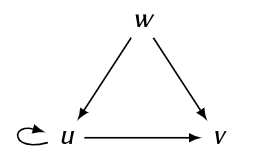
\includegraphics[width=.5\linewidth]{Assets/Systemsicherheit-acyclic-tam-example.png}

    Note: In bar,u is both a parent type (because of $s_1$) and a child type (because of $s_2$) $\rightarrow$  hence the loop edge.

    Safety Decidability: We call a TAM model acyclic, iff its TCG is acyclic.

    \note{Theorem 5}{Safety of a ternary, acyclic, monotonous TAM model (TAMTAM) is decidable in polynomial time in the size of $m_0$.}

    Crucial property acyclic, intuitively:
    \begin{itemize*}
        \item Evolution of the system (protection state transitions) checks both rights in the ACM as well as argument types
        \item TCG is acyclic $\Rightarrow\exists$ a finite sequence of possible state transitions after which no input tuple with argument types, that were not already considered before, can be found
        \item One may prove that an algorithm, which tries to expandall possible different follow-up states from $q_0$, may terminate after this finite sequence
    \end{itemize*}

    Expressive Power of TAMTAM
    \begin{itemize*}
        \item MTAM: obviously same expressive power as monotonic HRU
        \begin{itemize*}
            \item no transfer of rights: "take r ... in turn grant r to ..."
            \item no countdown rights: "r can only be used n times"
        \end{itemize*}
        \item ORCON: allow to ignore non-monotonic command $s$ from STS since they only remove rights and are reversible
        \item AMTAM: most MTAM STS may be re-written as acyclic
        \item TAMTAM: expressive power equivalent to AMTAM
    \end{itemize*}

    IBAC Model Comparison: family of IBAC models to describe different ranges of security policies they are able to express
    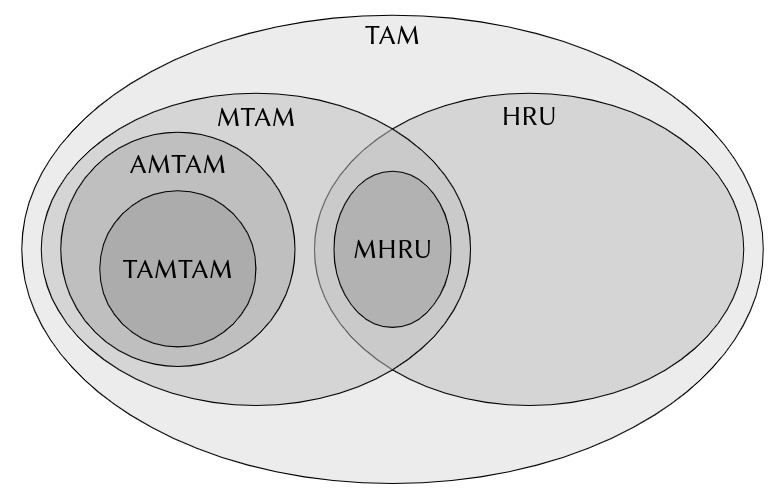
\includegraphics[width=.5\linewidth]{Assets/Systemsicherheit-ibac-model-comparison.png}

    IBAC Summary
    \begin{itemize*}
        \item Model identity-based AC policies (IBAC)
        \item Analyze them w.r.t. basic security properties (right proliferation)
        \item $\rightarrow$  Minimize specification errors
        \item $\rightarrow$  Minimize implementation errors
        \item Approach
        \begin{itemize*}
            \item Unambiguous policy representation through formal notation
            \item Prediction and/or verification of mission-critical properties
            \item Derivation of implementation concepts
        \end{itemize*}
        \item Model Range - Static models:
        \begin{itemize*}
            \item Access control function: $f:S\times O\times OP\rightarrow \{true,false\}$
            \item Access control matrix (ACM): $m:S\times O\rightarrow 2^{OP}$
            \item Static analysis: Which rights are assigned to whom, which (indirect) information flows are possible
            \item Implementation: Access control lists (ACLs)
        \end{itemize*}
        \item Model Range - Dynamic models:
        \begin{itemize*}
            \item ACM plus deterministic automaton $\rightarrow$ Analysis of dynamic behavior: HRU safety
            \item generally undecidable
            \item decidable under specific restrictions: monotonous mono-conditional, static, typed, etc.
            \item identifying and explaining safety-violations, in case such (are assumed to) exists: heuristic analysis algorithms
        \end{itemize*}
        \item Limitations
        \begin{itemize*}
            \item IBAC models are fundamental: KISS
            \item IBAC models provide basic expressiveness only
        \end{itemize*}
        \item For more application-oriented policy semantics:
        \begin{itemize*}
            \item Large information systems: many users, many databases, files, ... $\rightarrow$ Scalability problem
            \item Access decisions not just based on subjects, objects, and operations $\rightarrow$ Abstraction problem
        \end{itemize*}
    \end{itemize*}

    \subsubsection{Roles-based Access Control Models (RBAC)}
    Solving Scalability and Abstraction results in smaller modeling effort results in smaller chance of human errors made in the process
    \begin{itemize*}
        \item Improved scalability and manageability
        \item application-oriented semantic: $roles\approx functions$ in organizations
        \item Models include smart abstraction: roles
        \item AC rules are specified based on roles instead of identities
        \item Users, roles, and rights for executing operations
        \item Access rules are based onrolesof users $\rightarrow$ on assignments
    \end{itemize*}

    \note{Basic RBAC model ,,$RBAC_0$''}{An $RBAC_0$ model is a tuple $\langle U,R,P,S,UA,PA,user,roles\rangle$ where
        \begin{itemize*}
            \item U is a set of user identifiers,
            \item R is a set of role identifiers,
            \item P is a set of permission identifiers,
            \item S is a set of session identifiers,
            \item $UA\subseteq U\times R$ is a many-to-many user-role-relation,
            \item $PA\subseteq P\times R$ is a many-to-many permission-role-relation,
            \item $user:S\rightarrow U$ is a total function mapping sessions to users,
            \item $roles:S\rightarrow 2^R$ is a total function mapping sessions to sets of roles such that $\forall s\in S:r\in roles(s)\Rightarrow \langle user(s),r\rangle \in UA$.
        \end{itemize*}
    }

    Interpretation
    \begin{itemize*}
        \item Users U model people: actual humans that operate the AC system
        \item Roles R model functions, that originate from the workflows and areas of responsibility in organizations
        \item Permissions P model rights for any particular access to a particular document
        \item user-role-relation $UA\subseteq U\times R$ defines which roles are available to users at any given time $\rightarrow$ must be assumed during runtime first before they are usable!
        \item permission-role-relation $PA\subseteq P\times R$ defines which permissions are associate with roles
        \item $UA$ and $PA$ describe static policy rules: Roles available to a user are not considered to possibly change, same with permissions associated with a role.
        \item Sessions $S$ describe dynamic assignments of roles $\rightarrow$ a session $s\in S$ models when a user is logged in(where she may use some role(s) available to her as per $UA$):
        \begin{itemize*}
            \item The session-user-mapping user: $S\rightarrow U$ associates a session with its ("owning") user
            \item The session-roles-mapping roles: $S\rightarrow 2^R$ associates a session with the set of roles currently assumed by that user (active roles)
        \end{itemize*}
    \end{itemize*}

    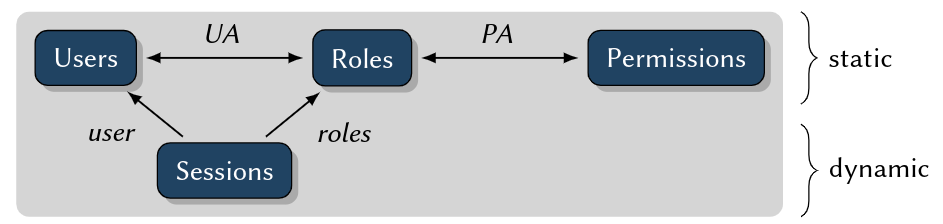
\includegraphics[width=.5\linewidth]{Assets/Systemsicherheit-rbac-0.png}

    \paragraph{RBAC Access Control Function}
    \begin{itemize*}
        \item access rules have to be defined for operations on objects
        \item implicitly defined through $P\rightarrow$ made explicit: $P\subseteq O\times OP$ is a set of permission tuples $\langle o,op\rangle$ where
        \begin{itemize*}
            \item $o\in O$ is an object from a set of object identifiers,
            \item $op\in OP$ is an operation from a set of operation identifiers.
        \end{itemize*}
        \item We may now define the $ACF$ for $RBAC_0$
    \end{itemize*}

    \note{$RBAC_0$ ACF}{
        $f_{RBAC_0}:U \times O\times OP\rightarrow\{true,false\}$ where

        $f_{RBAC_0} (u,o,op)= \begin{cases} true, \quad \exists r\in R,s\in S:u=user(s)\wedge r\in roles(s)\wedge \langle \langle o,op\rangle ,r\rangle  \in PA \\ false, \quad\text{ otherwise } \end{cases}$
    }

    \paragraph{RBAC96 Model Family}
    In practice, organizations have more requirements that need to be expressed in their security policy
    \begin{itemize*}
        \item Roles are often hierarchical $\rightarrow RBAC_1 = RBAC_0 + hierarchies$
        \item Role association and activation are often constrained $\rightarrow$ $RBAC_2 = RBAC_0 + constraints$
        \item Both may be needed $\rightarrow$ $RBAC_3$ = consolidation: $RBAC_0 + RBAC_1 + RBAC_2$
    \end{itemize*}

    \paragraph{RBAC 1: Role Hierarchies}
    Roles often overlap
    \begin{enumerate*}
        \item disjoint permissions for roles proManager and proDev $\rightarrow$ any proManager user must always have proDev assigned and activated for any of her workflows $\rightarrow$ role assignment redundancy
        \item overlapping permissions: $\forall p\in P:\langle p,proDev\rangle \in PA\Rightarrow \langle p,proManager\rangle \in PA\rightarrow$ any permission for project developers must be assigned to two different roles $\rightarrow$ role definition redundancy
        \item Two types of redundancy $\rightarrow$ undermines scalability goal of RBAC
    \end{enumerate*}

    Solution: Role hierarchy $\rightarrow$ Eliminates role definition redundancy through permissions inheritance

    Modeling Role Hierarchies
    \begin{itemize*}
        \item Lattice here: $\langle R,\leq\rangle$
        \item Hierarchy expressed through dominance relation: $r_1\leq r_2 \Leftrightarrow r_2$ inherits any permissions from $r_1$
        \item Interpretation
        \begin{itemize*}
            \item Reflexivity: any role consists of ("inherits") its own permissions
            \item Antisymmetry: no two different roles may mutually inherit their respective permissions
            \item Transitivity: permissions may be inherited indirectly
        \end{itemize*}
    \end{itemize*}

    \note{$RBAC_1$ Security Model}{An $RBAC_1$ model is a tuple $\langle U,R,P,S,UA,PA,user,roles,RH\rangle$ where
        \begin{itemize*}
            \item $U,R,P,S,UA,PA$ and $user$ are defined as for $RBAC_0$,
            \item $RH\subseteq R\times R$ is a partial order that represents a role hierarchy where $\langle r,r'\rangle \in RH\Leftrightarrow r\leq r'$ such that $\langle R,\leq\rangle$ is a lattice,
            \item roles is defined as for $RBAC_0$, while additionally holds: $\forall r,r'\in R,\exists s\in S:r\leq r'\wedge r'\in roles(s)\Rightarrow r\in roles(s)$.
        \end{itemize*}
    }

    \paragraph{RBAC 2 : Constraints}
    Assuming and activating roles in organizations is often more restricted:
    \begin{itemize*}
        \item Certain roles may not be active at the same time (same session) for any user
        \item Certain roles may not be together assigned to any user
        \item $\rightarrow$ separation of duty (SoD)
        \item While SoD constraints are a more fine-grained type of security requirements to avoid mission-critical risks, there are other types represented by RBAC constraints.
    \end{itemize*}
    Constraint Types
    \begin{itemize*}
        \item Separation of duty: mutually exclusive roles
        \item Quantitative constraints: maximum number of roles per user
        \item Temporal constraints: time/date/week/... of role activation
        \item Factual constraints: assigning or activating roles for specific permissions causally depends on any roles for a certain, other permissions
    \end{itemize*}
    Modeling Constraints Idea
    \begin{itemize*}
        \item $RBAC_2: \langle U,R,P,S,UA,PA,user,roles,RE\rangle$
        \item $RBAC_3: \langle U,R,P,S,UA,PA,user,roles,RH,RE\rangle$
        \item where $RE$ is a set of logical expressions over the other model components (such as $UA,PA,user,roles$)
    \end{itemize*}

    \paragraph{RBAC Summary}
    \begin{itemize*}
        \item Scalability
        \item Application-oriented model abstractions
        \item Standardization (RBAC96) $\rightarrow$ tool-support for:
        \begin{itemize*}
            \item role engineering (identifying and modeling roles)
            \item model engineering (specifying/validating a model config.)
            \item static model checking (verifying consistency and plausibility of a model configuration)
        \end{itemize*}
        \item Still weak OS-support
        \begin{itemize*}
            \item $\rightarrow$ application-level integrations
            \item $\rightarrow$ middleware integrations
        \end{itemize*}
        \item Limited dynamic analyses w.r.t. automaton-based models
    \end{itemize*}

    \subsubsection{Attribute-based Access Control Models}
    \begin{itemize*}
        \item Scalability and manageability
        \item Application-oriented model abstractions
        \item Model semantics meet functional requirements of open systems:
        \begin{itemize*}
            \item user IDs, INode IDs, ... only available locally
            \item roles limited to specific organizational structure; only assignable to users
        \end{itemize*}
        \item $\rightarrow$ Consider application-specific context of an access: attributes of subjects and objects(e. g. age, location, trust level, ...)
    \end{itemize*}

    Idea: Generalizing the principle of indirection already known from RBAC
    \begin{itemize*}
        \item IBAC: no indirection between subjects and objects
        \item RBAC: indirection via roles assigned to subjects
        \item ABAC: indirection via arbitrary attributes assigned to subjects or objects
        \item Attributes model application-specific properties of the system entities involved in any access
        \begin{itemize*}
            \item Age, location, trustworthiness of a application/user/...
            \item Size, creation time, access classification of resource/...
            \item Risk quantification involved with these subjects and objects
        \end{itemize*}
    \end{itemize*}

    \paragraph{ABAC Access Control Function}
    \begin{itemize*}
        \item $f_{IBAC}:S\times O\times OP\rightarrow\{true,false\}$
        \item $f_{RBAC}:U\times O\times OP\rightarrow\{true,false\}$
        \item $f_{ABAC}:S\times O\times OP\rightarrow\{true,false\}$
        \item $\rightarrow$ Evaluates attribute values for $\langle s,o,op\rangle$
    \end{itemize*}

    \paragraph{ABAC Security Model}
    \begin{itemize*}
        \item Note: There is no such thing (yet) like a standard ABAC model
        \item Instead: Many highly specialized, application-specific models.
        \item Here: minimal common formalism, based on Servos and Osborn
    \end{itemize*}

    \note{ABAC Security Model}{An ABAC security model is a tuple $\langle S,O,AS,AO,attS,attO,OP,AAR\rangle$ where
        \begin{itemize*}
            \item $S$ is a set of subject identifiers and $O$ is a set of object identifiers,
            \item $A_S=V_S^1 \times...\times V_S^n$ is a set of subject attributes, where each attribute is an n-tuple of values from arbitrary domains $V_S^i$, $1\leq i \leq n$,
            \item $A_O=V_O^1\times...\times V_O^m$ is a corresponding set of object attributes, based on values from arbitrary domains $V_O^j$, $1\leq j \leq m$,
            \item $att_S:S\rightarrow A_S$ is the subject attribute assignment function,
            \item $att_O:O\rightarrow A_O$ is the object attribute assignment function,
            \item $OP$ is a set of operation identifiers,
            \item $AAR\subseteq \Phi\times OP$ is the authorization relation.
        \end{itemize*}
    }

    Interpretation
    \begin{itemize*}
        \item Active and passive entities are modeled by $S$ and $O$, respectively
        \item Attributes in $AS,AO$ are index-referenced tuples of values, which are specific to some property of subjects $V_S^i$ (e.g. age) or of objects $V_O^j$ (e. g. PEGI rating)
        \item Attributes are assigned to subjects and objects via $att_S,att_O$
        \item Access control rules w.r.t. the execution of operations in $OP$ are modeled by the $AAR$ relation $\rightarrow$ determines ACF!
        \item $AAR$ is based on a set of first-order logic predicates $\Phi$: $\Phi=\{\phi_1 (x_{s1},x_{o1}),\phi_2 (x_{s2},x_{o2}),...\}$. Each $\phi_i\in\Phi$ is a binary predicate, where $x_{si}$ is a subject variable and $x_{oi}$ is an object variable.
    \end{itemize*}

    \note{ABAC Access Control Function (ACF)}{
        \begin{itemize*}
            \item $f_{ABAC}:S\times O\times OP\rightarrow\{true,false\}$ where
            \item $f_{ABAC}(s,o,op)= \begin{cases} true, \quad\exists \langle \phi,op\rangle \in AAR:\phi(s,o)=true\\ false, \quad\text{ otherwise } \end{cases}$.
            \item We call $\phi$ an authorization predicate for $op$.
        \end{itemize*}
    }

    \paragraph{ABAC Summary}
    \begin{itemize*}
        \item Scalability
        \item Application-oriented model abstractions
        \item Universality: ABAC can conveniently express IBAC, RBAC, MLS
        \item Still weak OS-support $\rightarrow$ application-level integrations
        \item Attribute semantics highly diverse, not normalizable $\rightarrow$ no common ,,standard ABAC''
        \item Limited dynamic analyses w.r.t. automaton-based models
    \end{itemize*}

    \subsubsection{Information Flow Models}
    Abstraction Level of AC Models: rules about subjects accessing objects. Adequate for
    \begin{itemize*}
        \item Workflow systems
        \item Document/information management systems
    \end{itemize*}

    Goal of Information Flow (IF) Models: Problem-oriented definition of policy rules for scenarios based on information flows(rather than access rights)

    Lattices (refreshment)
    \begin{itemize*}
        \item $inf_C$: ,,systemlow''
        \item $sup_C$: ,,systemhigh''
        \item has a source: $deg^-(inf_C)= 0$
        \item has a sink: $deg^+(sup_C)= 0$
    \end{itemize*}

    Implementation of Information Flow Models
    \begin{itemize*}
        \item Information flows and read/write operations are isomorphic
        \begin{itemize*}
            \item s has read permission o $\Leftrightarrow$ information may flow from o to s
            \item s has write permission o $\Leftrightarrow$ information may flow from s to o
        \end{itemize*}
        \item $\rightarrow$ Implementation by standard AC mechanisms!
    \end{itemize*}

    Analysis of Information Flow Models
    \begin{itemize*}
        \item IF Transitivity $\rightarrow$ goal: covert information flows
        \item IF Antisymmetry $\rightarrow$ goal: redundancy
    \end{itemize*}

    \note{Denning Security Model}{A Denning information flow model is a tuple $\langle S,O,L,cl,\bigoplus\rangle$ where
        \begin{itemize*}
            \item S is a set of subjects,
            \item O is a set of objects,
            \item $L=\langle C,\leq\rangle$ is a lattice where
            \begin{itemize*}
                \item C is a set of classes,
                \item $\leq$ is a dominance relation where c $\leq d \Leftrightarrow$ information may flow from c to d,
            \end{itemize*}
            \item $cl:S\cup O\rightarrow C$ is a classification function, and
            \item $\bigoplus:C\times C\rightarrow C$ is a reclassification function.
        \end{itemize*}
    }

    Interpretation
    \begin{itemize*}
        \item Subject set S models active entities, which information flows originate from
        \item Object set O models passive entities, which may receive information flows
        \item Classes set C used to label entities with identical information flow properties
        \item Classification function $cl$ assigns a class to each entity
        \item Reclassification function $\bigoplus$ determines which class an entity is assigned after receiving certain a information flow
    \end{itemize*}

    We can now ...
    \begin{itemize*}
        \item precisely define all information flows valid for a given policy
        \item define analysis goals for an IF model w.r.t.
        \begin{itemize*}
            \item Correctness: $\exists$ covert information flows? (transitivity of $\leq$, automation: graph analysis tools)
            \item Redundancy: $\exists$ sets of subjects and objects with (transitively) equivalent information contents? (antisymmetry of $\leq$, automation: graph analysis tools)
        \end{itemize*}
        \item implement a model: through an automatically generated, isomorphic ACM(using already-present ACLs!)
    \end{itemize*}

    \paragraph{Multilevel Security (MLS)}
    \begin{itemize*}
        \item Introducing a hierarchy of information flow classes: levels of trust
        \item Subjects and objects are classified:
        \begin{itemize*}
            \item Subjects w.r.t. their trust worthiness
            \item Objects w.r.t. their criticality
        \end{itemize*}
        \item Within this hierarchy, information may flow only in one direction $\rightarrow$ ,,secure'' according to these levels!
        \item $\rightarrow \exists$ MLS models for different security goals!
    \end{itemize*}

    Modeling Confidentiality Levels
    \begin{itemize*}
        \item Class set: levels of confidentiality e.g. $C=\{public,conf,secret\}$
        \item Dominance relation: hierarchy between confidentiality levels e.g. $\{public \leq confidential,confidential \leq secret\}$
        \item Classification of subjects and objects: $cl:S\cup O\rightarrow C$ e.g. $cl(BulletinBoard)=public,cl(Timetable)=confidential$
        \item In contrast due Denning $\leq$ in MLS models is a total order
    \end{itemize*}

    \paragraph{The Bell-LaPadula Model}
    MLS-Model for Preserving Information Confidentiality.
    Incorporates impacts on model design ...
    \begin{itemize*}
        \item from the application domain: hierarchy of trust
        \item from the Denning model: information flow and lattices
        \item from the MLS models: information flow hierarchy
        \item from the HRU model:
        \begin{itemize*}
            \item Modeling dynamic behavior: state machine and STS
            \item Model implementation: ACM
        \end{itemize*}
        \item $\rightarrow$ application-oriented model engineering by composition of known abstractions
    \end{itemize*}

    Idea:
    \begin{itemize*}
        \item entity sets S,O
        \item $lattice\langle C,\leq\rangle$ defines information flows by
        \begin{itemize*}
            \item C: classification/clearance levels
            \item $\leq$: hierarchy of trust
        \end{itemize*}
        \item classification function $cl$ assigns
        \begin{itemize*}
            \item clearance level from C to subjects
            \item classification level from C to objects
        \end{itemize*}
        \item Model’s runtime behavior is specified by a deterministic automaton
    \end{itemize*}

    \note{BLP Security Model}{A BLP model is a deterministic automaton $\langle S,O,L,Q,\sum,\sigma,q_0,R\rangle$ where
        \begin{itemize*}
            \item S and O are (static) subject and object sets,
            \item $L=\langle C,\leq\rangle$ is a (static) lattice consisting of
            \begin{itemize*}
                \item the classes set C,
                \item the dominance relation $\leq$,
            \end{itemize*}
            \item $Q=M\times CL$ is the state space where
            \begin{itemize*}
                \item $M=\{m|m:S\times O\rightarrow 2^R\}$ is the set of possible ACMs,
                \item $CL=\{cl|cl:S\cup O\rightarrow C\}$ is a set of functions that classify entities in $S\cup O$,
            \end{itemize*}
            \item $\sum$ is the input alphabet,
            \item $\sigma:Q\times \sum\rightarrow Q$ is the state transition function,
            \item $q_0\in Q$ is the initial state,
            \item $R=\{read,write\}$ is the set of access rights.
        \end{itemize*}
    }

    Interpretation
    \begin{itemize*}
        \item $S,O,M,\sum,\sigma,q_0,R$: same as HRU
        \item L: models confidentiality hierarchy
        \item cl: models classification meta-information about subjects and objects
        \item $Q=M\times CL$ models dynamic protection states; includes
        \begin{itemize*}
            \item rights in the ACM,
            \item classification of subjects/objects,
            \item not: S and O (different to HRU)
        \end{itemize*}
        \item Commands in the STS may therefore
        \begin{itemize*}
            \item change rights in the ACM,
            \item reclassify subjects and objects.
        \end{itemize*}
    \end{itemize*}
    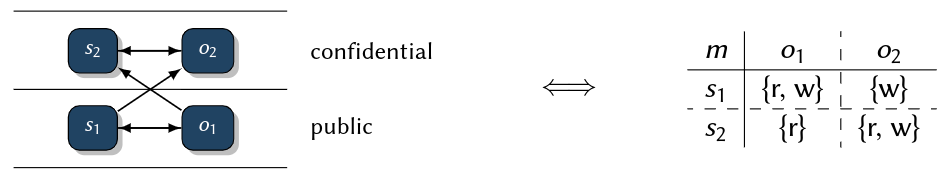
\includegraphics[width=\linewidth]{Assets/Systemsicherheit-lattice-vs-acm.png}

    \begin{itemize*}
        \item L is an application-oriented abstraction
        \begin{itemize*}
            \item Supports convenient for model specification
            \item Supports easy model correctness analysis
            \item $\rightarrow$ easy to specify and to analyze
        \end{itemize*}
        \item m can be directly implemented by standard OS/DBIS access control mechanisms (ACLs, Capabilities) $\rightarrow$ easy to implement
        \item m is determined (= restricted) by L and cl, not vice-versa
        \item L and cl control m
        \item m provides an easy specification for model implementation
    \end{itemize*}

    \subsubsection{BLP Security}
    \note{Read-Security Rule}{A BLP model state $\langle m,cl\rangle$ is called read-secure iff $\forall s\in S,o\in O:read\in m(s,o)\Rightarrow cl(o) \leq cl(s)$.}

    \note{Write-Security Rule}{A BLP model state $\langle m,cl\rangle$ is called write-secure iff $\forall s\in S,o\in O:write\in m(s,o)\Rightarrow cl(s)\leq cl(o)$.}

    \note{State Security}{A BLP model state is called secure iff it is both read- and write-secure.}

    \note{Model Security}{A BLP model with initial state $q_0$ is called secure iff
        \begin{enumerate*}
            \item $q_0$ is secure and
            \item each state reachable from $q_0$ by a finite input sequence is secure.
        \end{enumerate*}
    }

    Auxiliary Definition: The Basic Security Theorem for BLP (BLP BST)
    \begin{itemize*}
        \item A convenient tool for proving BLP security
        \item Idea: let’s look at properties of the finite and small model components $\rightarrow\sigma\rightarrow$ STS
    \end{itemize*}

    \note{The BLP Basic Security Theorem}{A BLP model $\langle S,O,L,Q,\sum,\sigma,q_0,R\rangle$ is secure iff both of the following holds:
        \begin{enumerate*}
            \item $q_0$ is secure
            \item $\sigma$ is build such that for each state q reachable from $q_0$ by a finite input sequence, where $q=\langle m,cl\rangle$ and $q'=\sigma(q,\delta)=m',cl',\forall s\in S, o\in O,\delta\in\sum$ the following holds:
        \end{enumerate*}
        \begin{itemize*}
            \item Read-security conformity:
            \begin{itemize*}
                \item read $\not\in m(s,o)\wedge read\in m'(s,o)\Rightarrow cl'(o)\leq cl'(s)$
                \item read $\in m(s,o) \wedge\lnot (cl'(o)\leq cl'(s)) \Rightarrow read \not\in m'(s,o)$
            \end{itemize*}
            \item Write-security conformity:
            \begin{itemize*}
                \item write $\not\in m(s,o)\wedge write \in m'(s,o)\Rightarrow cl'(s)\leq cl'(o)$
                \item write $\in m(s,o)\wedge\lnot(cl'(s)\leq cl'(o)) \Rightarrow write \not\in m'(s,o)$
            \end{itemize*}
        \end{itemize*}
    }

    Proof of Read Security
    \begin{itemize*}
        \item Let $q=\sigma*(q_0 ,\sigma^+),\sigma^+\in\sigma^+,q'=\delta(q,\sigma),\sigma\in\sigma,s\in S,o\in O$. With $q=\langle m,cl\rangle$ and $q'=m',cl'$, the BLP BST for read-security
        \begin{itemize*}
            \item (a1) $read \not\in m(s,o) \wedge read\in m'(s,o) \Rightarrow cl'(o) \leq cl'(s)$
            \item (a2) $read \in m(s,o) \wedge\lnot (cl'(o)\leq cl'(s)) \Rightarrow read \not\in m'(s,o)$
            \item Let’s first introduce some convenient abbreviations for this:
            \begin{itemize*}
                \item $R:=read\in m(s,o)$
                \item $R':=read\in m'(s,o)$
                \item $C':=cl'(o) \leq cl'(s)$
                \item $\sigma^+$ is the set of finite, non-empty input sequences.
            \end{itemize*}
            \item Proposition: $(a1) \wedge (a2)\equiv read-security$
            \item Proof: $(a1) \wedge (a2)= R' \Rightarrow C'\equiv read\in m'(s,o) \Rightarrow cl'(o)\leq cl'(s)$, which exactly matches the definition of read-security for $q'$.
            \item Write-security: Same steps for $(b1)\wedge (b2)$.
        \end{itemize*}
    \end{itemize*}

    Idea: Encode an additional, more fine-grained type of access restriction in the ACM $\rightarrow$ compartments
    \begin{itemize*}
        \item Comp: set of compartments
        \item $co:S\cup O\rightarrow 2^{Comp}$: assigns a set of compartments to an entity as an (additional) attribute
        \item Refined state security rules:
        \begin{itemize*}
            \item $\langle m,cl,co\rangle$ is read-secure $\Leftrightarrow\forall s\in S,o\in O:read \in m(s,o)\Rightarrow cl(o)\leq cl(s)\wedge co(o) \subseteq co(s)$
            \item $\langle m,cl,co\rangle$ is write-secure $\Leftrightarrow\forall s\in S,o\in O:write\in m(s,o)\Rightarrow cl(s)\leq cl(o)\wedge co(o) \subseteq co(s)$
        \end{itemize*}
        \item old BLP: $\langle S,O,L,Q,\sigma,\delta,q_0\rangle$
        \item With compartments: $\langle S,O,L,Comp,Q_{co},\sigma,\delta,q_0\rangle$ where $Q_{co}=M\times CL\times CO$ and $CO=\{co|co:S\cup O\rightarrow 2^{Comp}\}$
    \end{itemize*}

    Example
    \begin{itemize*}
        \item Let $co(o)=secret,co(o)=airforce$
        \item $s_1$ where $cl(s_1)=public,co(s_1)=\{airforce,navy\}$ can write o
        \item $s_2$ where $cl(s_2)=secret,co(s_2)=\{airforce,navy\}$ read/write o
        \item $s_3$ where $cl(s_3)=secret,co(s_3)=\{navy\}$ can do neither
    \end{itemize*}


    \paragraph{BLP Model Summary}
    \begin{itemize*}
        \item Application-oriented modeling $\rightarrow$ hierarchical information flow
        \item Scalability $\rightarrow$ attributes: trust levels
        \item Modeling dynamic behavior $\rightarrow$ automaton with STS
        \item Correctness guarantees (analysis of)
        \begin{itemize*}
            \item consistency: BLP security, BST
            \item completeness of IF: IFG path finding
            \item presence of unintended IF: IFG path finding
            \item unwanted redundancy: IF cycles
            \item safety properties: decidable
        \end{itemize*}
        \item Implementation
        \begin{itemize*}
            \item ACM is a standard AC mechanism in contemporary implementation platforms (cf. prev. slide)
            \item Contemporary standard OSs need this: do not support mechanisms for entity classification, arbitrary STSs
            \item new platforms: SELinux, TrustedBSD, PostgreSQL, ...
        \end{itemize*}
        \item Is an example of a hybrid model: IF + AC + ABAC
    \end{itemize*}

    learn from BLP for designing and using security models
    \begin{itemize*}
        \item Model composition from known model abstractions
        \begin{itemize*}
            \item Denning: IF modeling
            \item ABAC: IF classes and compartments as attributes
            \item MSL: modeling trust as a linear hierarchy
            \item HRU: modeling dynamic behavior
            \item ACM: implementing application-oriented policy semantics
        \end{itemize*}
        \item Consistency is an important property of composed models
        \item BLP is further extensible and refinable
    \end{itemize*}

    \subsubsection{The Biba Model}
    BLP upside down

    \begin{center}
        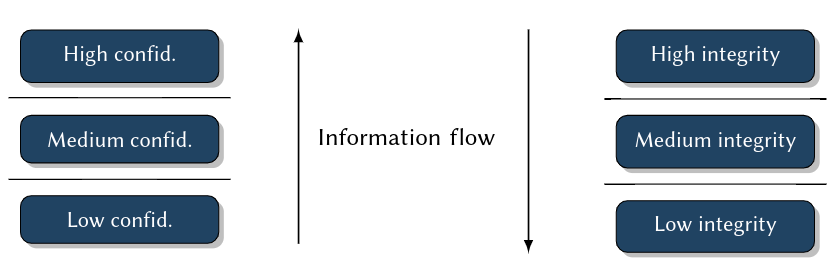
\includegraphics[width=.5\linewidth]{Assets/Systemsicherheit-blp-vs-biba.png}
    \end{center}
    \begin{itemize*}
        \item BLP $\rightarrow$ preserves confidentiality
        \item Biba $\rightarrow$ preserves integrity
    \end{itemize*}

    OS Example
    \begin{itemize*}
        \item Integrity: Protect system files from malicious user/software
        \item Class hierarchy (system, high, medium, low)
        \item every file/process/... created is classified $\rightarrow$ cannot violate integrity of objects
        \item Manual user involvement: resolving intended exceptions, e.g. install trusted application
    \end{itemize*}


    \subsubsection{Non-interference Models}
    Problems: Covert Channels \& Damage Range (Attack Perimeter)

    \note{Covert Channel}{Channels not intended for information transfer at all, such as the service program’s effect on the system load.}

    \begin{itemize*}
        \item AC policies (ACM, HRU, TAM, RBAC, ABAC): colluding malware agents, escalation of common privileges
        \begin{itemize*}
            \item Process 1: only read permissions on user files
            \item Process 2: only permission to create an internet socket
            \item both: communication via covert channel
        \end{itemize*}
        \item MLS policies (Denning, BLP, Biba): indirect information flow exploitation (can never prohibitany possible transitive IF ...)
        \begin{itemize*}
            \item Test for existence of a file
            \item Volume control on smartphones
            \item Timing channels from server response times
        \end{itemize*}
    \end{itemize*}

    Idea of NI models
    \begin{itemize*}
        \item higher level of abstraction
        \item Policy semantics: which domains should be isolated based on their mutual impact
    \end{itemize*}

    Consequences
    \begin{itemize*}
        \item Easier policy modeling
        \item More difficult policy implementation $\rightarrow$ higher degree of abstraction
    \end{itemize*}

    Example
    \begin{itemize*}
        \item Fields: Smart Cards, Server System
        \item Different services, different providers, different levels of trust
        \item Shared resources
        \item Needed: isolation of services, restricted cross-domain interactions
        \item $\rightarrow$ Guarantee of total/limited non-interference between domains
    \end{itemize*}

    \paragraph{NI Security Policies}
    Specify
    \begin{itemize*}
        \item Security domains
        \item Cross-domain (inter)actions $\rightarrow$ interference
    \end{itemize*}
    From convert channels to domain interference:
    \note{Non-Interference}{Two domains do not interfere with each other iff no action in one domain can be observed by the other.}

    \note{NI Security Model}{An NI model is a det. automaton $\langle Q,\sigma,\delta,\lambda,q_0,D,A,dom,\approx_{NI},Out\rangle$ where
        \begin{itemize*}
            \item Q is the set of (abstract) states,
            \item $\sigma=A$ is the input alphabet where A is the set of (abstract) actions,
            \item $\delta:Q\times\sigma\rightarrow Q$ is the state transition function,
            \item $\lambda:Q\times\sigma\rightarrow Out$ is the output function,
            \item $q_0\in Q$ is the initial state,
            \item $D$ is a set of domains,
            \item $dom:A\rightarrow 2^D$ is adomain function that completely defines the set of domains affected by an action,
            \item $\approx_{NI}\subseteq D\times D$ is a non-interference relation,
            \item $Out$ is a set of (abstract) outputs.
        \end{itemize*}
        NI Security Model is also called Goguen/Meseguer-Model.
    }

    BLP written as an NI Model
    \begin{itemize*}
        \item BLP Rules:
        \begin{itemize*}
            \item write in class public may affect public and confidential
            \item write in class confidential may only affect confidential
        \end{itemize*}
        \item NI Model:
        \begin{itemize*}
            \item $D=\{d_{pub},d_{conf}\}$
            \item write in $d_{conf}$ does not affect $d_{pub}$, so $d_{conf} \approx_{NI} d_{pub}$
            \item $A=\{writeInPub, writeInConf\}$
            \item $dom(writeInPub)=\{d_{pub},d_{conf}\}$
            \item $dom(writeInConf)=\{d_{conf}\}$
        \end{itemize*}
    \end{itemize*}

    \paragraph{NI Model Analysis}
    Goals
    \begin{itemize*}
        \item AC models: privilege escalation ($\rightarrow$ HRU safety)
        \item BLP models: model consistency ($\rightarrow$ BLP security)
        \item NI models: Non-interference between domains
    \end{itemize*}

    \note{Purge Function}{Let $aa^*\in A^*$ be a sequence of actions consisting of a single action $a\in A\cup\{\epsilon\}$ followed by a sequence $a^*\in A^*$, where $\epsilon$ denotes an empty sequence. Let $D'\in 2^D$ be any set of domains. Then, purge: $A^*\times 2^D \rightarrow A^*$ computes a subsequence of $aa^*$ by removing such actions without an observable effect on any element of $D':$
        \begin{itemize*}
            \item $purge(aa^*,D')=\begin{cases} a\circ purge(a^*,D'), \quad\exists d_a\in dom(a),d'\in D':d_a\approx_I d' \\ purge(a^*,D'), \quad\text{ otherwise }\end{cases}$
            \item $purge(\epsilon,D')=\epsilon$
        \end{itemize*}
        where $\approx_I$ is the complement of $\approx_{NI}:d_1 \approx_I d_2\Leftrightarrow \lnot(d_1 \approx_{NI} d_2)$.
    }

    \note{NI Security}{For a state $q\in Q$ of an NI model $\langle Q,\sigma,\delta,\lambda,q_0,D,A,dom,\approx_{NI},Out\rangle$, the predicate ni-secure (q) holds iff $\forall a\in A,\forall a^*\in A^*:\lambda (\delta^*(q,a^*),a)=\lambda(\delta^*(q,purge(a^*,dom(a))),a)$.}

    Interpretation
    \begin{enumerate*}
        \item Running an NI model on $\langle q,a^*\rangle$ yields $q'=\delta^*(q,a^*)$.
        \item Running the model on the purged input sequence so that it contains only actions that, according to $\approx_{NI}$, actually have impact on $dom(a)$ yields $q'_{clean}=\delta^*(q,purge(a^*,dom(a)))$
        \item If $\forall a\in A:\lambda(q',a)=\lambda(q'_{clean},a)$, than the model is called NI-secure w.r.t. q($ni-secure(q)$).
    \end{enumerate*}

    \paragraph{Comparison to HRU and IF Models}
    \begin{itemize*}
        \item HRU Models
        \begin{itemize*}
            \item Policies describe rules that control subjects accessing objects
            \item Analysis goal: right proliferation
            \item Covert channels analysis: only based on model implementation
        \end{itemize*}
        \item IF Models
        \begin{itemize*}
            \item Policies describe rules about legal information flows
            \item Analysis goals: indirect IFs, redundancy, inner consistency
            \item Covert channel analysis: same as HRU
        \end{itemize*}
        \item NI Models
        \begin{itemize*}
            \item Rules about mutual interference between domains
            \item Analysis goal: consistency of $\approx_{NI}$ and $dom$
            \item Implementation needs rigorous domain isolation (e.g. object encryption is not sufficient) $\rightarrow$ expensive
            \item State of the Art w.r.t. isolation completeness
        \end{itemize*}
    \end{itemize*}

    \subsubsection{Hybrid Models}
    \paragraph{Chinese-Wall Policies}
    for consulting companies
    \begin{itemize*}
        \item Clients of any such company
        \begin{itemize*}
            \item Companies, including their business data
            \item Often: mutual competitors
        \end{itemize*}
        \item Employees of consulting companies
        \begin{itemize*}
            \item Are assigned to clients they consult
            \item Work for many clients $\rightarrow$ gather insider information
        \end{itemize*}
        \item Policy goal: No flow of (insider) information between competing clients
    \end{itemize*}

    Why look at specifically these policies? Modeling
    \begin{itemize*}
        \item Composition of
        \begin{itemize*}
            \item Discretionary IBAC components
            \item Mandatory ABAC components
        \end{itemize*}
        \item Driven by real-world demands: iterative refinements of a model over time
        \begin{itemize*}
            \item Brewer-Nash model
            \item Information flow model
            \item Attribute-based model
        \end{itemize*}
        \item Application areas: consulting, cloud computing
    \end{itemize*}

    \paragraph{The Brewer-Nash Model}
    Explicitly tailored towards Chinese Wall (CW) policies

    Model Abstractions
    \begin{itemize*}
        \item Consultants represented by subjects
        \item Client companies represented by objects, which comprise a company’s business data
        \item Modeling of competition by conflict classes: two different clients are competitors $\Leftrightarrow$ their objects belong to the same class
        \item No information flow between competing objects $\rightarrow$ a ,,wall'' separating any two objects from the same conflict class
        \item Additional ACM for refined management settings of access permissions
    \end{itemize*}

    Representation of Conflict Classes
    \begin{itemize*}
        \item Client company data: object set O
        \item Competition: conflict relation $C\subseteq O\times O:\langle o,o'\rangle \in C\Leftrightarrow o$ and $o'$ belong to competing companies (non-reflexive, symmetric, generally not transitive)
        \item In terms of ABAC:object attribute $att_O:O\rightarrow 2^O$, such that $att_O(o)=\{o'\in O|\langle o,o'\rangle \in C\}$.
    \end{itemize*}

    Representation of a Consultant’s History
    \begin{itemize*}
        \item Consultants: subject set S
        \item History relation $H\subseteq S\times O:\langle s,o\rangle \in H\Leftrightarrow s$ has previously consulted $o$
        \item In terms of ABAC: subject attribute $att_S:S\rightarrow 2^O$, such that $att_S(s)=\{o\in O|\langle s,o\rangle \in H\}$.
    \end{itemize*}

    \note{Brewer-Nash Security Model}{The Brewer-Nash model of the CW policy is a det. $automaton\langle S,O,Q,\sigma,\delta,q_0,R\rangle$ where
        \begin{itemize*}
            \item $S$ and $O$ are sets of subjects (consultants) and (company data) objects,
            \item $Q=M\times 2^C\times 2^H$ is the state space where
            \begin{itemize*}
                \item $M=\{m|m:S\times O\rightarrow 2^R\}$ is the set of possible ACMs,
                \item $C\subseteq O\times O$ is the conflict relation: $\langle o,o'\rangle \in C\Leftrightarrow o$ and $o'$ are competitors,
                \item $H\subseteq S\times O$ is the history relation: $\langle s,o\rangle \in H\Leftrightarrow s$ has previously
                consulted $o$,
            \end{itemize*}
            \item $\sigma=OP \times X$ is the input alphabet where
            \begin{itemize*}
                \item $OP=\{read,write\}$ is a set of operations,
                \item $X=S \times O$ is the set of arguments of these operations,
            \end{itemize*}
            \item $\delta:Q \times\sigma\rightarrow Q$ is the state transition function,
            \item $q_0\in Q$ is the initial state,
            \item $R=\{read,write\}$ is the set of access rights.
        \end{itemize*}
    }

    \paragraph{Brewer-Nash STS}
    \begin{itemize*}
        \item Read (similar to HRU notation)
        command read(s,o)::=if read $\in$ m(s,o) $\wedge\forall \langle o',o\rangle \in C:\langle s,o'\rangle \not\in H$
        then
        $H:=H\cup\{\langle s,o\rangle \}$
        fi
        \item Write
        command write(s,o)::=if write $\in$ m(s,o) $\wedge\forall o'\in O:o'\not=o \Rightarrow \langle s,o'\rangle \not\in H$
        then
        $H:=H\cup\{\langle s,o\rangle \}$
        fi
    \end{itemize*}

    Not shown: Discretionary policy portion $\rightarrow$ modifications in m to enable fine-grained rights management.

    Restrictiveness
    \begin{itemize*}
        \item Write Command: s is allowed to write $o\Leftrightarrow write\in m(s,o)\wedge\forall o'\in O:o'\not=o\Rightarrow\langle s,o'\rangle \not\in H$
        \item Why so restrictive? $\rightarrow$ No transitive information flow!
        \item $\rightarrow$ s must never have previously consulted any other client!
        \item any consultant is stuck with her client on first read access
    \end{itemize*}

    \paragraph{Brewer-Nash Model}
    \begin{itemize*}
        \item Initial State $q_0$
        \begin{itemize*}
            \item $m_0$: consultant assignments to clients, issued by management
            \item $C_0$: according to real-life competition
            \item $H_0 =\varnothing$
        \end{itemize*}
    \end{itemize*}

    \note{Secure State}{$\forall o,o' \in O,s\in S:\langle s,o\rangle \in H_q\wedge\langle s,o'\rangle \in H_q\Rightarrow\langle o,o'\rangle \not\in C_q$

        Corollary: $\forall o,o'\in O,s\in S:\langle o,o'\rangle \in C_q\wedge\langle s,o\rangle \in H_q\Rightarrow \langle s,o'\rangle \not\in H_q$
    }

    \note{Secure Brewer-Nash Model}{Similar to ,,secure BLP model''.}

    \paragraph{Summary Brewer-Nash}
    What’s remarkable with this model?
    \begin{itemize*}
        \item Composes DAC and MAC components
        \item Simple model paradigms
        \begin{itemize*}
            \item Sets (subjects, objects)
            \item ACM (DAC)
            \item Relations (company conflicts, consultants history)
            \item Simple ,,read'' and ,,write'' rule
            \item $\rightarrow$ easy to implement
        \end{itemize*}
        \item Analysis goals
        \begin{itemize*}
            \item MAC: Model security
            \item DAC: safety properties
        \end{itemize*}
        \item Drawback: Restrictive write-rule
    \end{itemize*}

    Professionalization
    \begin{itemize*}
        \item Remember the difference: trusting humans (consultants) vs. trusting software agents (subjects)
        \begin{itemize*}
            \item Consultants are assumed to be trusted
            \item Systems (processes, sessions, ...) may fail
        \end{itemize*}
        \item $\rightarrow$ Write-rule applied not to humans, but to software agents
        \item $\rightarrow$ Subject set S models consultant’s subjects (e.g. processes) in a group model
        \begin{itemize*}
            \item All processes of one consultant form a group
            \item Group members
            \begin{itemize*}
                \item have the same rights in m
                \item have individual histories
                \item are strictly isolated w.r.t. IF
            \end{itemize*}
        \end{itemize*}
    \end{itemize*}

    \paragraph{The Least-Restrictive-CW Model}

    Restrictiveness of Brewer-Nash Model:
    \begin{itemize*}
        \item If $\langle o_i,o_k\rangle \in C$: no transitive information flow $o_i \rightarrow o_j\rightarrow o_k$, i.e. consultant(s) of $o_i$ must never write to any $o_j\not=o_i$
        \item This is actually more restrictive than necessary: $o_j\rightarrow o_k$ and afterwards $o_i\rightarrow o_j$ would be fine
        \item Criticality of an IF depends on existence of earlier flows.
    \end{itemize*}

    Idea LR-CW: Include time as a model abstraction!
    \begin{itemize*}
        \item $\forall s\in S,o\in O$: remember, which information has flown to entity
        \item $\rightarrow$ subject-/object-specific history, $\approx$attributes (,,lables'')
    \end{itemize*}

    \note{LR-CW Model}{The Least-Restrictive model of the CW policy is a deterministic $automaton \langle S,O,F,\zeta,Q,\sigma,\delta,q_0\rangle$ where
        \begin{itemize*}
            \item S and O are sets of subjects (consultants) and data objects,
            \item F is the set of client companies,
            \item $\zeta:O\rightarrow F$ (,,zeta'') function mapping each object to its company,
            \item $Q=2^C \times 2^H$ is the state space where
            \begin{itemize*}
                \item $C\subseteq F\times F$ is the conflict relation: $\langle f,f'\rangle \in C\Leftrightarrow f$ and $f'$ are competitors,
                \item $H=\{Z_e\subseteq F|e\in S\cup O\}$ is the history set: $f\in Z_e\Leftrightarrow e$ contains information about $f(Z_e$ is the ,,history label'' of $e$),
            \end{itemize*}
            \item $\sigma=OP\times X$ is the input alphabet where
            \begin{itemize*}
                \item $OP=\{read,write\}$ is the set of operations,
                \item $X=S\times O$ is the set of arguments of these operations,
            \end{itemize*}
            \item $\delta:Q\times\sigma\rightarrow Q$ is the state transition function,
            \item $q_0\in Q$ is the initial state
        \end{itemize*}
    }

    Inside the STS
    \begin{itemize*}
        \item a reading operation: requires that no conflicting information is accumulated in the subject potentially increases the amount of information in the subject
        \item a writing operation: requires that no conflicting information is accumulated in the object potentially increases the amount of information in the object
    \end{itemize*}

    Model Achievements
    \begin{itemize*}
        \item Applicability: more writes allowed in comparison to Brewer-Nash
        \item Paid for with
        \begin{itemize*}
            \item Need to store individual attributes of all entities (history labels)
            \item Dependency of write permissions on earlier actions of other subjects
        \end{itemize*}
        \item More extensions:
        \begin{itemize*}
            \item Operations to modify conflict relation
            \item Operations to create/destroy entities
        \end{itemize*}
    \end{itemize*}

    \subsubsection{An MLS Model for Chinese-Wall Policies}
    Conflict relation is
    \begin{itemize*}
        \item non-reflexive: no company is a competitor of itself
        \item symmetric: competition is always mutual
        \item not necessarily transitive: any company might belong to more than one conflict class $\rightarrow$ Cannot be modeled by a lattice
    \end{itemize*}

    Idea: Labeling of entities
    \begin{itemize*}
        \item Class of an entity (subject or object) reflects information it carries
        \item Consultant reclassified whenever a company data object is read
        \item $\rightarrow$ Classes and labels:
        \item Class set of a lattice $C=\{DB,Citi,Shell,Esso\}$
        \item Entity label: vector of information already present in each business branch
        \item In example, a vector consists of 2 elements $\in C$ resulting in labels as:
        \begin{itemize*}
            \item $[\epsilon,\epsilon]$ (exclusively for $inf_C$)
            \item $[DB,\epsilon]$ (for DB-objects or -consultants)
            \item $[DB,Shell]$ (for subjects or objects containing information from both DB and Shell)
        \end{itemize*}
    \end{itemize*}

    Why is the ,,Chinese Wall'' policy interesting?
    \begin{itemize*}
        \item One policy, multiple models:
        \item Brewer-Nash model demonstrates hybrid DAC-/MAC-/IFC-approach
        \item Least-Restrictive CW model demonstrates a more practical professionalization
        \item MLS-CW model demonstrates applicability of lattice-based IF modeling $\rightarrow$ semantically cleaner approach
        \item Applications: Far beyond traditional consulting scenarios...$\rightarrow$ current problems in cloud computing!
    \end{itemize*}

    \subsection{Summary - Security Models}
    \begin{itemize*}
        \item Formalize informal security policies for the sake of
        \begin{itemize*}
            \item objectification by unambiguous calculi
            \item explanation and proof of security properties by formal analysis techniques
            \item foundation for correct implementations
        \end{itemize*}
        \item Are composed of simple building blocks (e.g. ACMs, sets, relations, functions, lattices, state machines) that are combined and interrelated to form more complex models
    \end{itemize*}

    \section{Practical Security Engineering}
    Goal: Design of new, application-specific models
    \begin{itemize*}
        \item Identify common components $\rightarrow$ generic model core
        \item Core specialization
        \item Core extension
        \item Glue between model components
    \end{itemize*}

    \subsection{Model Engineering}
    Model Engineering Principles
    \begin{itemize*}
        \item Core model
        \item Core specialization
        \item Core extension
        \item Component glue
    \end{itemize*}

    Core Model (Common Model Core)
    \begin{itemize*}
        \item HRU: $\langle  Q, \sum , \delta, q_0  , \not R \rangle$
        \item $DRBAC_0$ : $\langle  Q, \sum , \delta, q_0  , \not R, \not P, \not PA \rangle$
        \item DABAC: $\langle  \not A , Q ,\sum , \delta, q_0  \rangle$
        \item TAM: $\langle  Q , \sum , \delta, q_0  , \not T, \not R \rangle$
        \item BLP: $\langle  \not S, \not O, \not L, Q , \sum , \delta, q_0  , \not R \rangle$
        \item NI: $\langle  Q , \sum , \delta, \not \lambda ,q_0  , \not D, \not A, \not dom, \not =_{NI} , \not Out \rangle$
        \item $\rightarrow  \langle  Q ,\sum , \delta, q_0  \rangle$
    \end{itemize*}

    Core Specialization
    \begin{itemize*}
        \item HRU: $\langle  Q, \sum , \delta, q_0  , R \rangle  \Rightarrow Q = 2^S \times  2^O \times M$
        \item $DRBAC_0$ : $\langle  Q, \sum , \delta, q_0  , R, P, PA \rangle  \Rightarrow Q = 2^U\times 2^{UA}\times 2^S \times  USER \times  ROLES$
        \item DABAC: $\langle  A , Q ,\sum , \delta, q_0  \rangle  \Rightarrow Q = 2^S\times 2^O \times M\times ATT$
        \item TAM: $\langle  Q , \sum , \delta, q_0  , T, R \rangle  \Rightarrow Q = 2^S\times 2^O\times TYPE \times M$
        \item BLP: $\langle  S, O, L, Q , \sum , \delta, q_0  , R \rangle  \Rightarrow Q = M \times CL$
        \item NI: $\langle  Q , \sum , \delta, \lambda ,q_0  , D, A, dom, =_{NI} , Out \rangle$
    \end{itemize*}

    Core Extensions
    \begin{itemize*}
        \item HRU: $\langle  Q, \sum , \delta, q_0  , R \rangle  \Rightarrow R$
        \item $DRBAC_0$ : $\langle  Q, \sum , \delta, q_0  , R, P, PA \rangle  \Rightarrow R,P,PA$
        \item DABAC: $\langle  A , Q ,\sum , \delta, q_0  \rangle  \Rightarrow A$
        \item TAM: $\langle  Q , \sum , \delta, q_0  , T, R \rangle  \Rightarrow T,R$
        \item BLP: $\langle  S, O, L, Q , \sum , \delta, q_0  , R \rangle  \Rightarrow S,O,L,R$
        \item NI: $\langle  Q , \sum , \delta, \lambda ,q_0  , D, A, dom, =_{NI} , Out \rangle  \Rightarrow \lambda,D,A,dom,=_{NI},Out$
        \item $\rightarrow R, P, PA, A , T , S , O , L , D , dom , =_{NI} , ...$
    \end{itemize*}

    Glue
    \begin{itemize*}
        \item E.g. TAM: State transition scheme (types)
        \item E.g. DABAC: State transition scheme (matrix and predicates)
        \item E.g. Brewer/Nash Chinese Wall model: ,,$\wedge$'' (simple, because $H+C\not= m$)
        \item E.g. BLP (much more complex, because rules restrict m by L and cl )
        \begin{itemize*}
            \item BLP read rule
            \item BLP write rule
            \item BST
        \end{itemize*}
    \end{itemize*}

    \subsection{Model Specification}
    Policy Implementation
    \begin{itemize*}
        \item We want: A system controlled by a security policy
        \item We have: A (satisfying) formal model of this policy
        \item How to convert a formal model into an executable policy? $\rightarrow$ Policy specification languages
        \item How to enforce an executable policy in a system? $\rightarrow$ security mechanisms and architectures
    \end{itemize*}

    Role of Specification Languages: Same as in software engineering
    \begin{itemize*}
        \item To bridge the gap between
        \begin{itemize*}
            \item Abstractions of security models (sets, relations, ...)
            \item Abstractions of implementation platforms (security mechanisms such as ACLs, krypto-algorithms,...)
        \end{itemize*}
        \item Foundation for Code verification or even more convenient: Automated code generation
    \end{itemize*}

    Approach
    \begin{itemize*}
        \item Abstraction level: Step stone between model and security mechanisms
        \item $\rightarrow$  More concrete than models
        \item $\rightarrow$  More abstract than programming languages (,,what'' instead of ,,how'')
        \item Expressive power: Domain-specific, for representing security models only
        \item $\rightarrow$  Necessary: adequate language paradigms
        \item $\rightarrow$  Sufficient: not more than necessary (no dead weight)
    \end{itemize*}

    Domains
    \begin{itemize*}
        \item Model domain, e.g. AC/IF/NI models (TAM, RBAC, ABAC)
        \item Implementation domain (OS, Middleware, Applications)
    \end{itemize*}


    \subsection{Model Specification }
    \subsubsection{CorPS}
    \subsubsection{SELinux Policy Language}
    \subsection{Summary}

    \section{Security Mechanisms}
    \subsection{Authorization}
    \subsubsection{Access Control Lists}
    \subsubsection{Capability Lists}
    \subsubsection{Interceptors}
    \subsubsection{Summary}
    \subsection{Cryptographic Mechanisms}
    \subsubsection{Encryption}
    \paragraph{Symmetric}
    \paragraph{Asymmetric}
    \subsubsection{Cryptographic Hashing}
    \subsubsection{Digital Signatures}
    \subsubsection{Cryptographic Attacks}
    \subsection{Identification and Authentication}
    \subsubsection{Passwords}
    \subsubsection{Biometrics}
    \subsubsection{Cryptographic Protocols}
    \paragraph{SmartCards}
    \paragraph{Authentication Protocols}
    \subsection{Summary}

    \section{Security Architectures}
    \subsection{Design Principles}
    \subsection{Operating Systems Architectures}
    \subsubsection{Nizza}
    \subsubsection{SELinux }
    \subsection{Distributed Systems Architectures}
    \subsubsection{CORBA }
    \subsubsection{Web Services }
    \subsubsection{Kerberos }
    \subsection{Summary}
\end{multicols}
\end{document}